\section{Graphics and Plots}

\subsection{Introduction and Theory}

\begin{figure}[h]
	\centering
	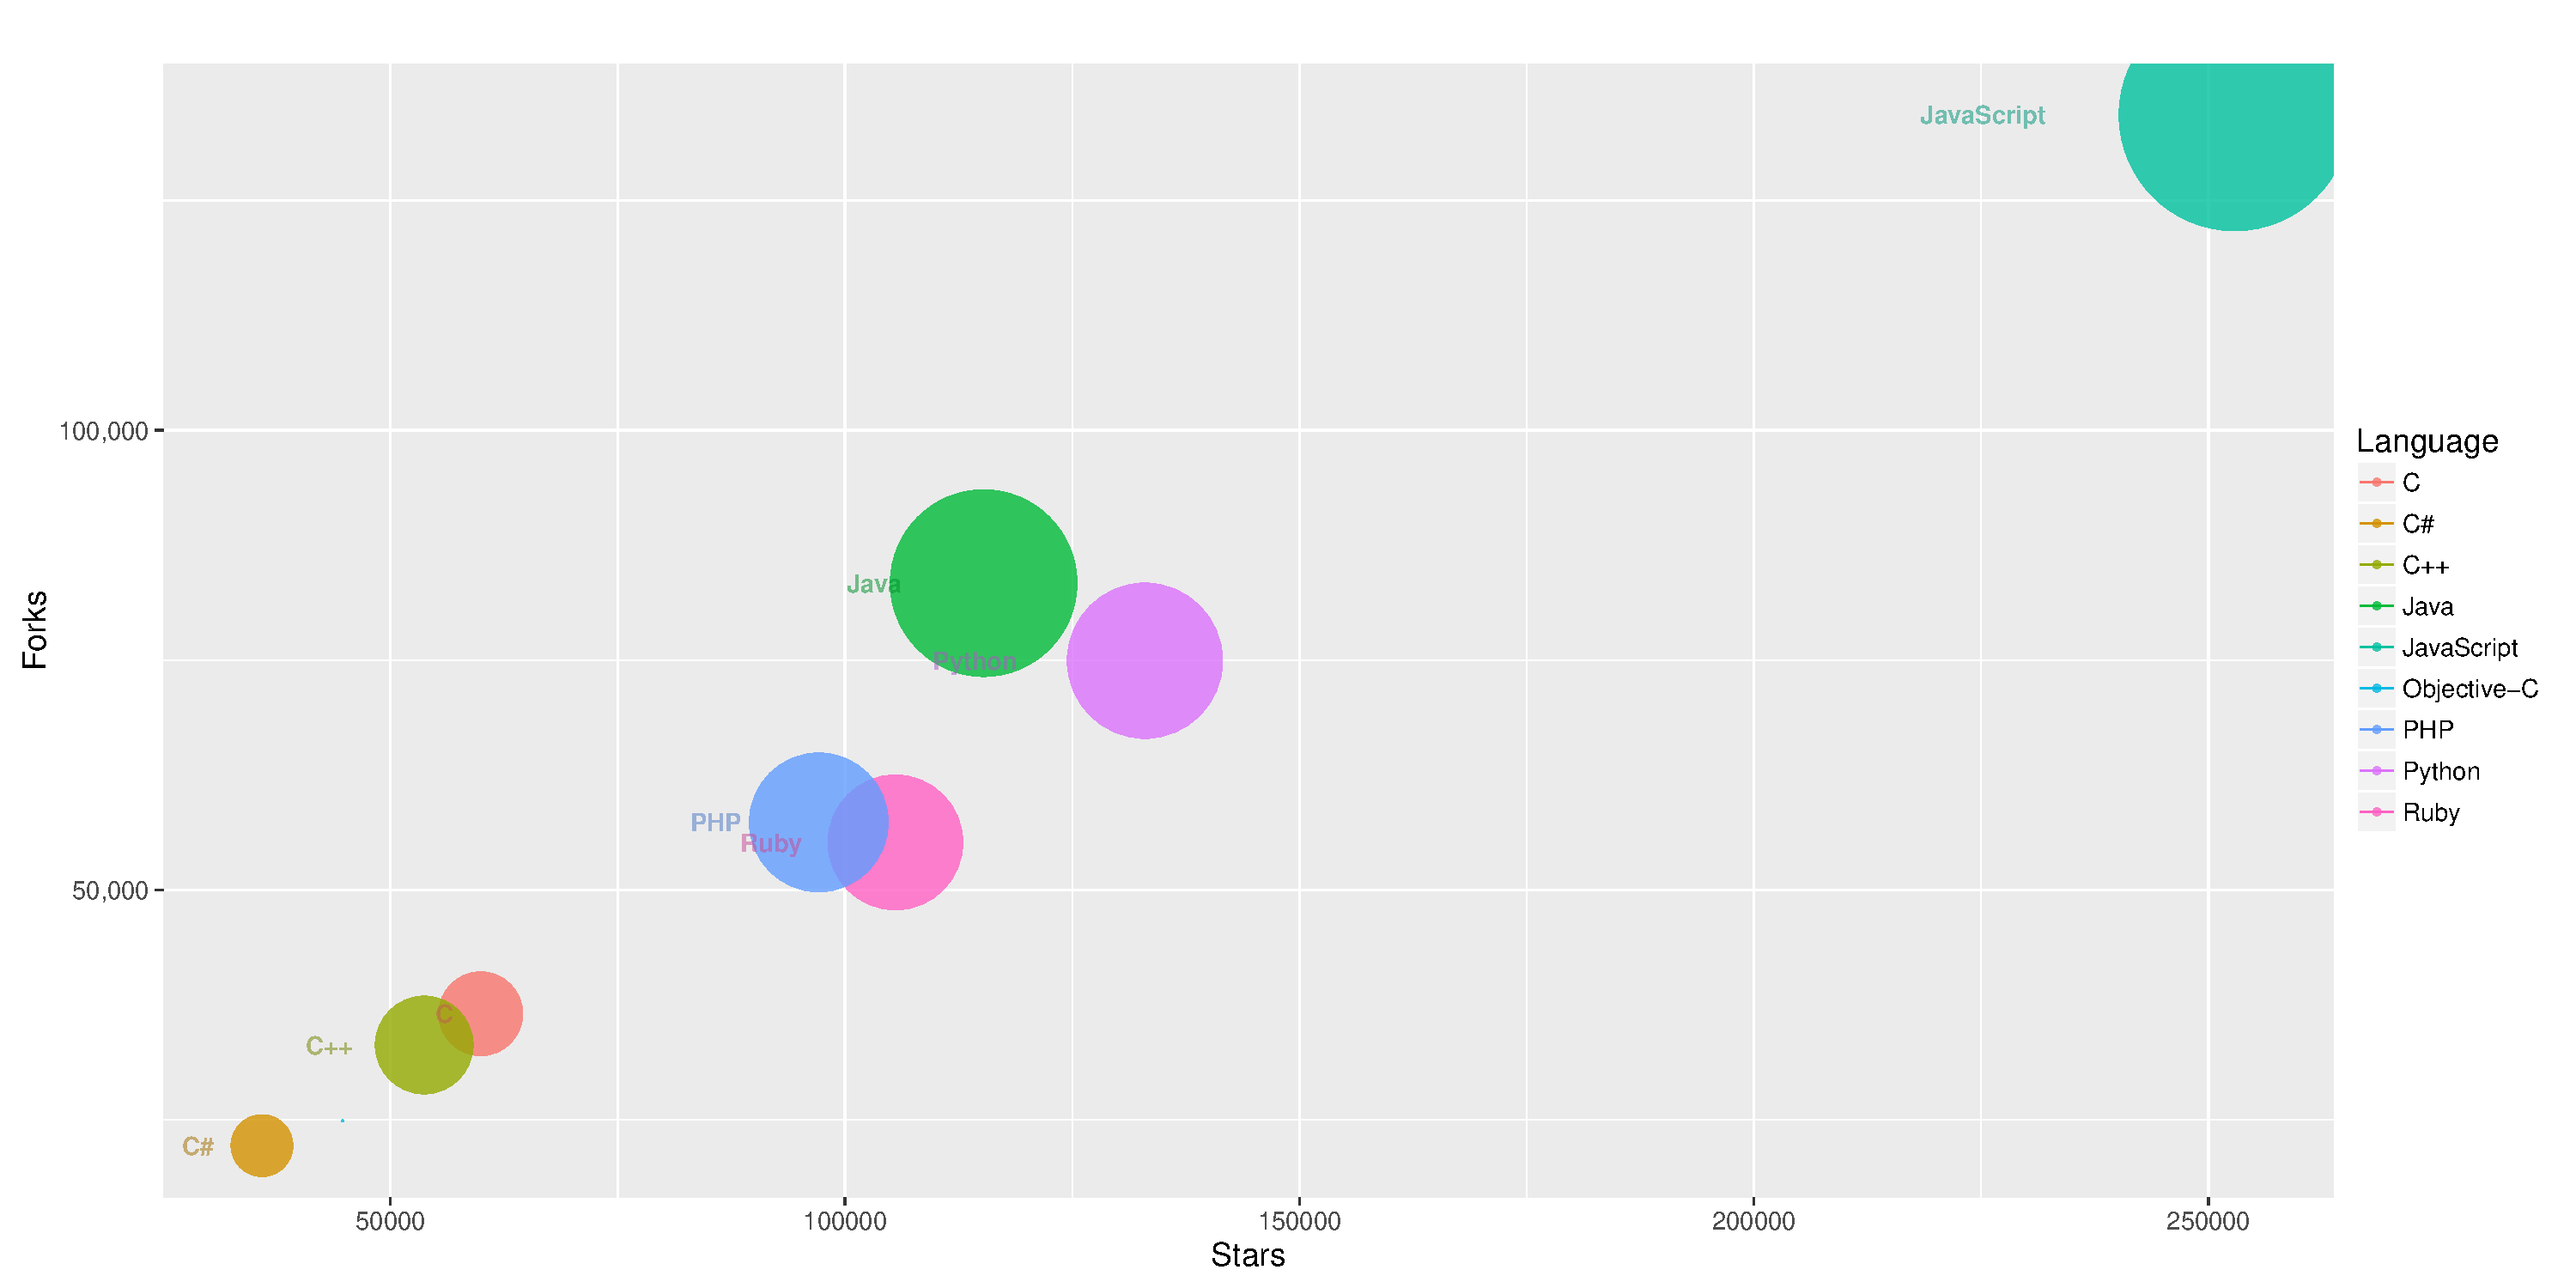
\includegraphics[page=1,scale=0.35]{../graphics/intro/popular_programming_languages.pdf}
	\caption[]{ Most popular languages on GitHub in 2014. The cumulated numbers of forks and stars on all projects can be regarded as proxy for the popularity of the programming language. The size of the circles represents the number of existing projects (proportions: JavaScript contains 323,938 projects, C\# contains 56,062 projects) \footnotemark}
	\label{fig:github_popular_programming_languages}
\end{figure}

\footnotetext{Data origin: \url{http://githut.info/}}

\begin{figure}[h]
	\centering
	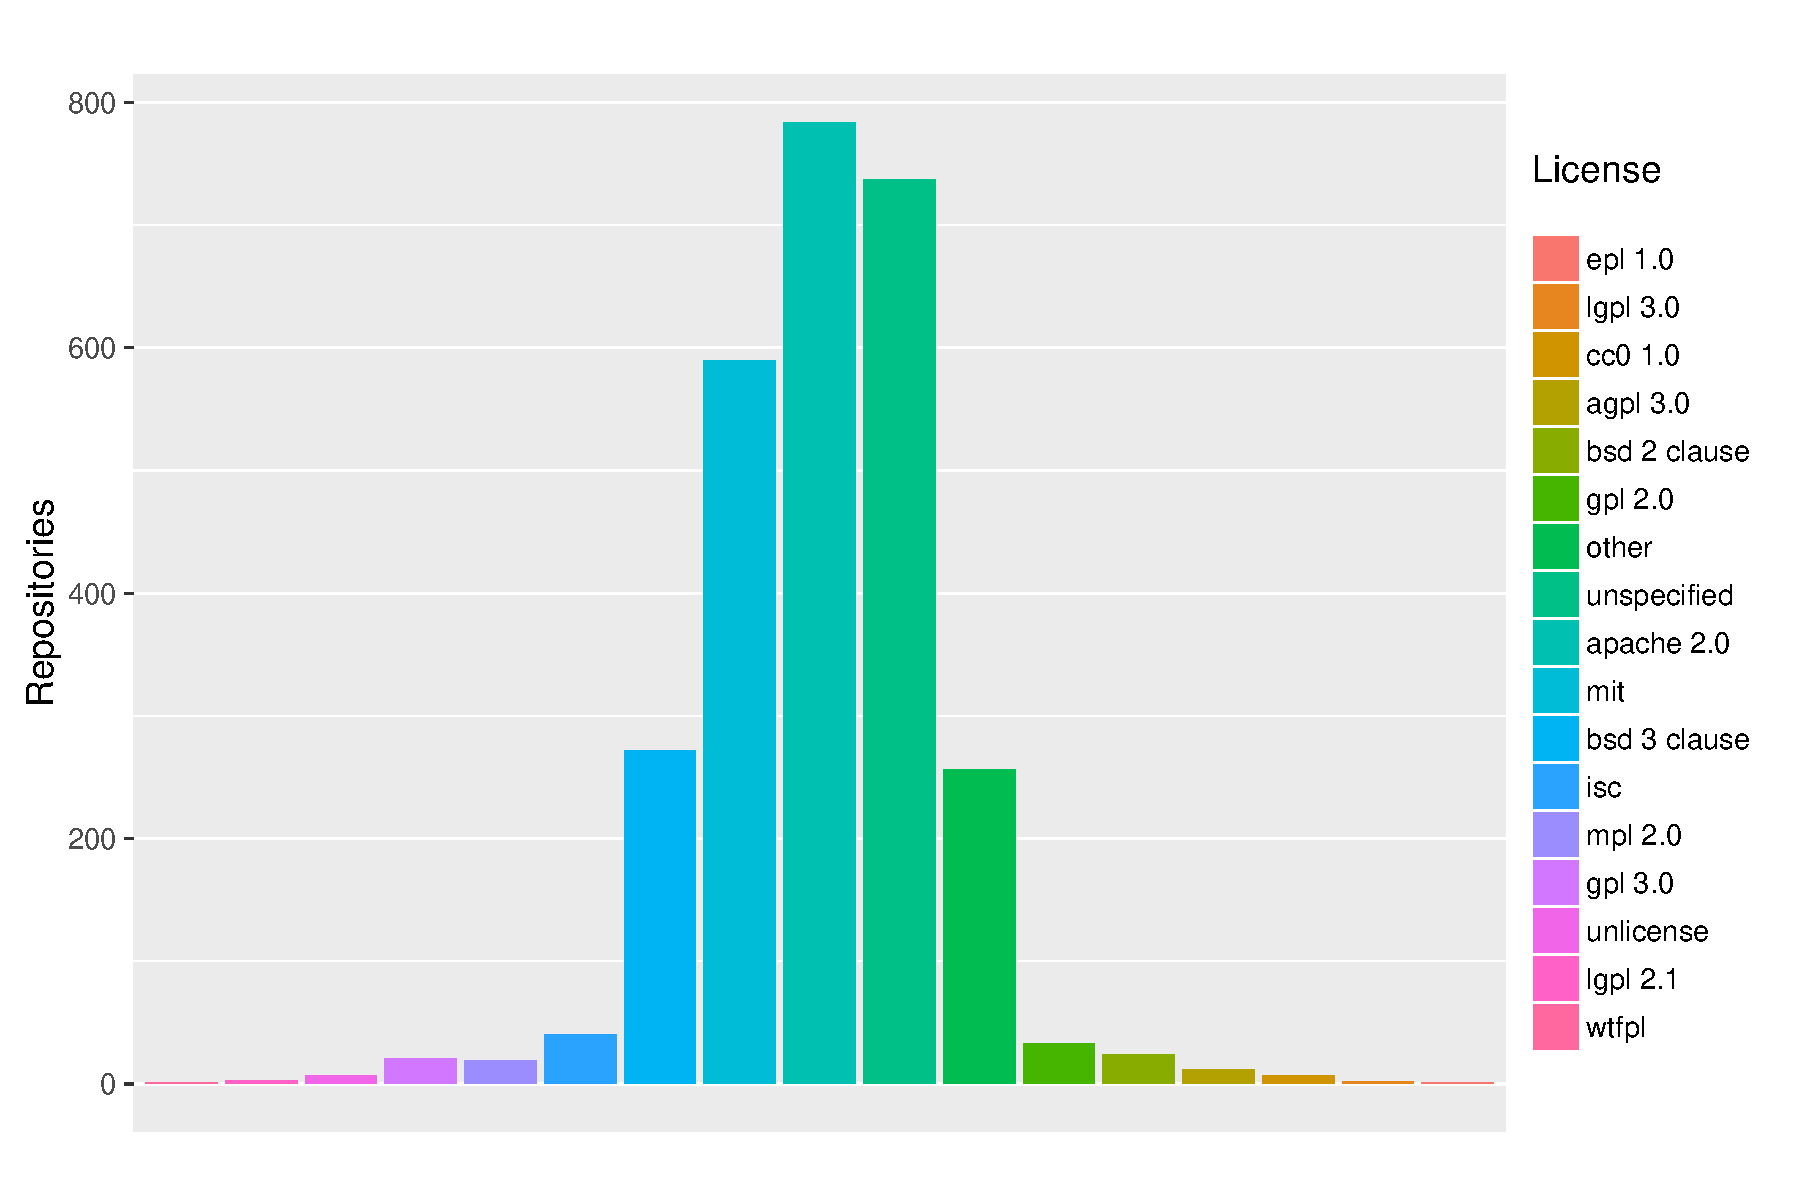
\includegraphics[page=1,scale=0.35]{../graphics/intro/licenses/popular_licenses_residual.pdf}
	\caption{License distribution of firm's residual projects on GitHub.}
	\label{fig:licenses_in_residual_projects}
\end{figure}

\begin{figure}[h]
	\centering
	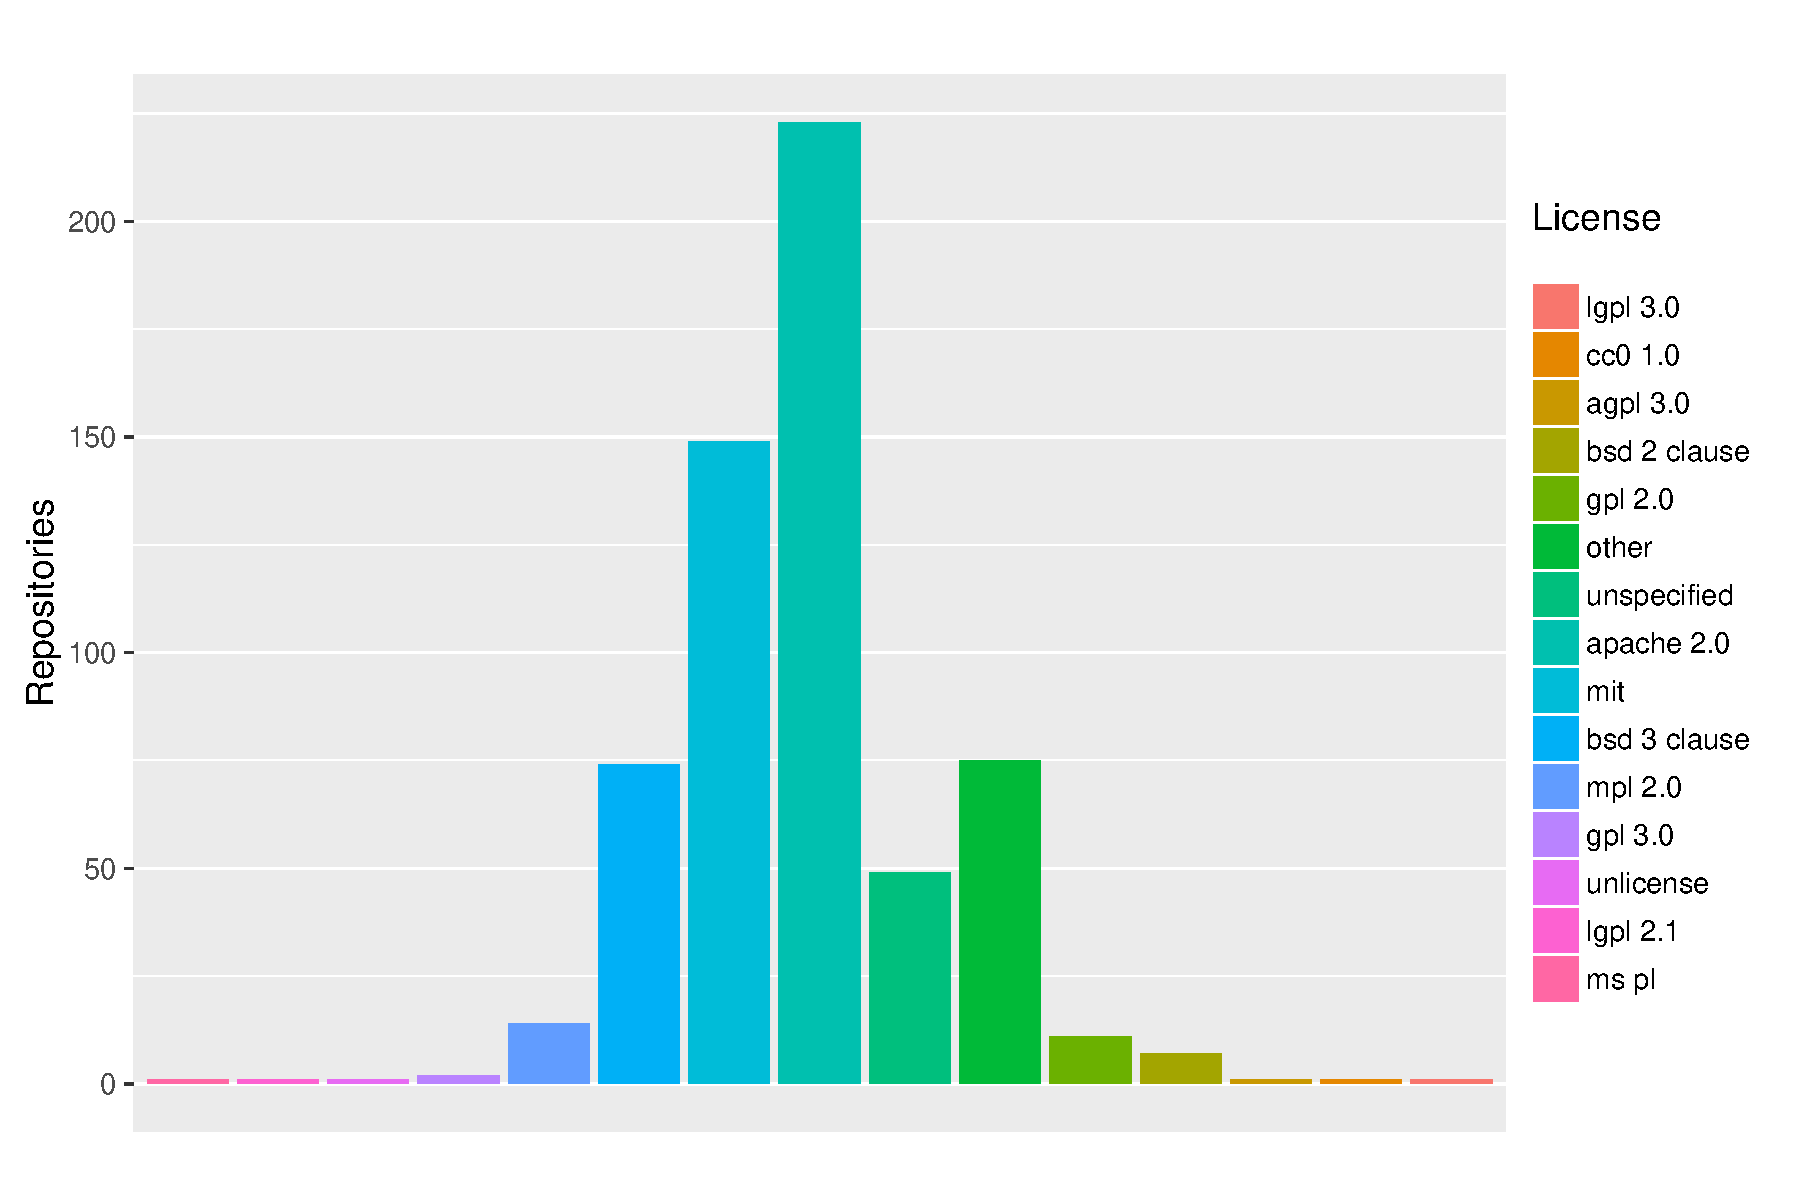
\includegraphics[page=1,scale=0.35]{../graphics/intro/licenses/popular_licenses_top.pdf}
	\caption{License distribution of firm's top projects on GitHub.}
	\label{fig:licenses_in_top_projects}
\end{figure}

\clearpage
\subsection{Plots of Code Contribution}

\begin{figure}[!ht]
	\centering
	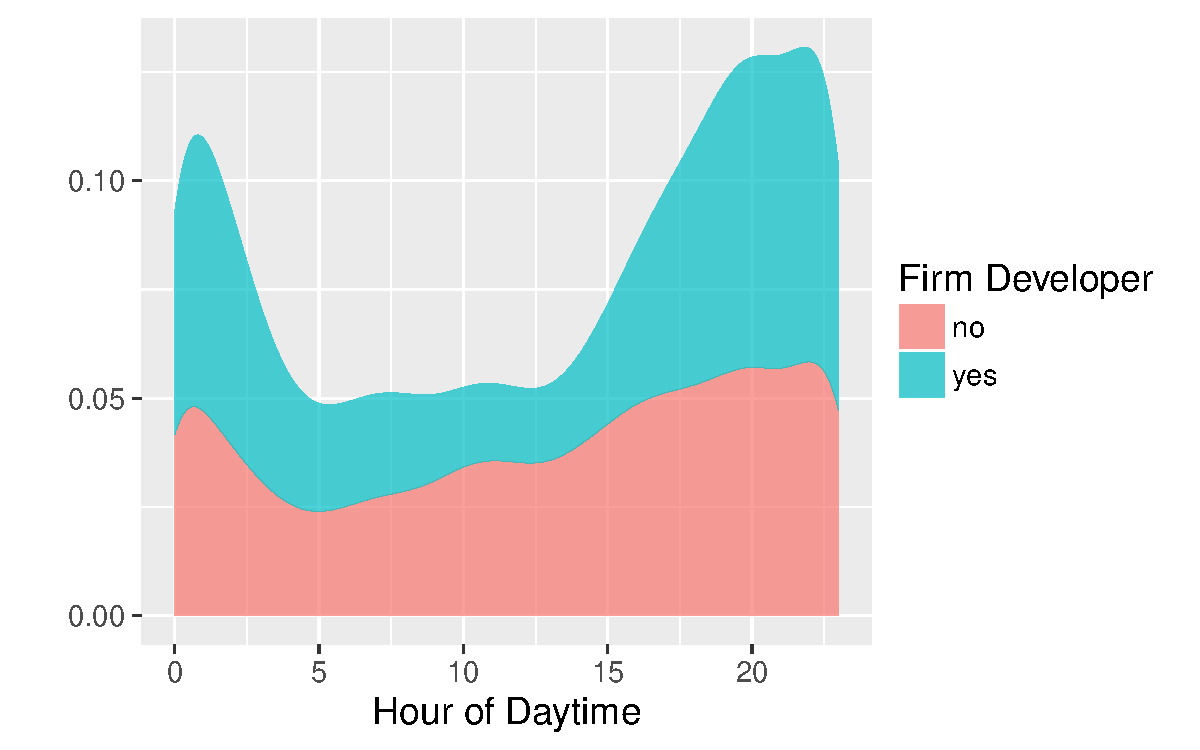
\includegraphics[page=1,scale=0.7]{../graphics/intro/hour_of_code_contribution_daytime_worldtime.pdf}
	\caption{Code contributions by firm employed and external developers based on worldwide consideration (UTC time). Most commits are placed during the late evening which is between morning and midday (9:00 - 16:00) in California, USA (UTC -8)}
	\label{fig:distribution_developer_commits_wordlwide}
\end{figure}

\begin{figure}[!ht]
	\centering
	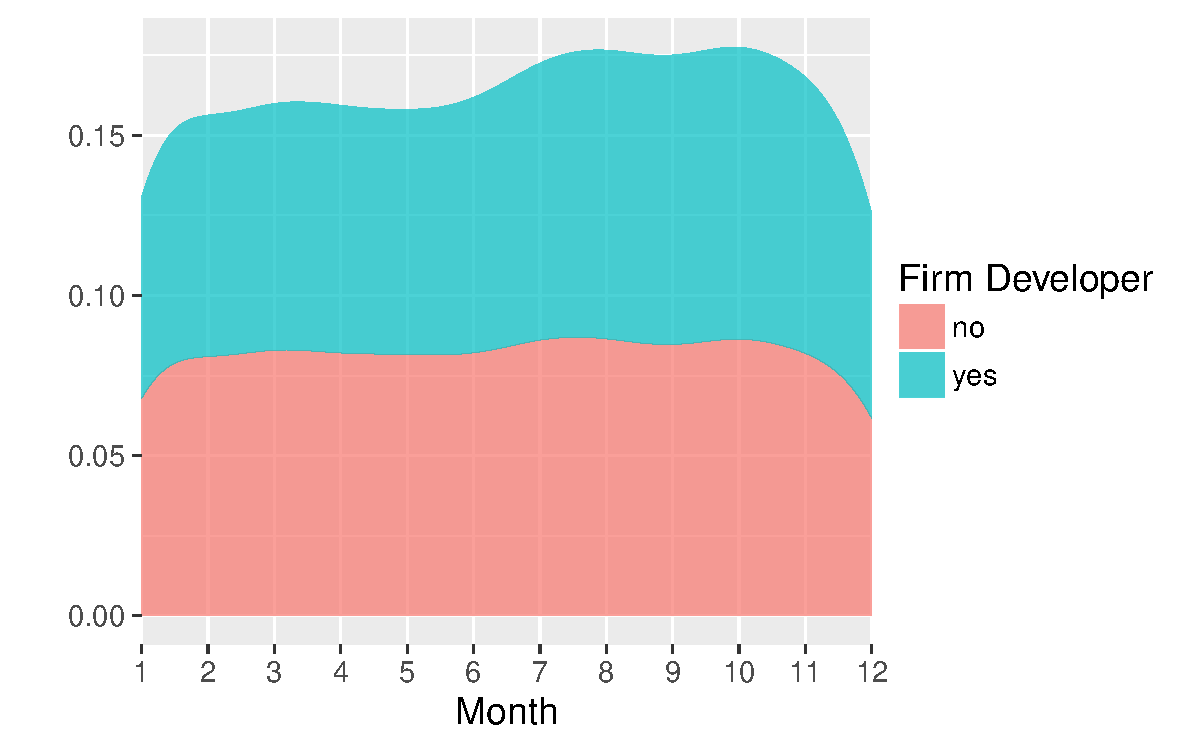
\includegraphics[page=1,scale=0.7]{../graphics/intro/month_of_code_contribution.pdf}
	\caption{Code contributions by firm employed and external developers over the year (January - December)}
	\label{fig:distribution_developer_commits_by_month}
\end{figure}

\subsection{Plots of Repositories}

\begin{figure}[h]
	\centering
	\label{fig:stars_contributors}
	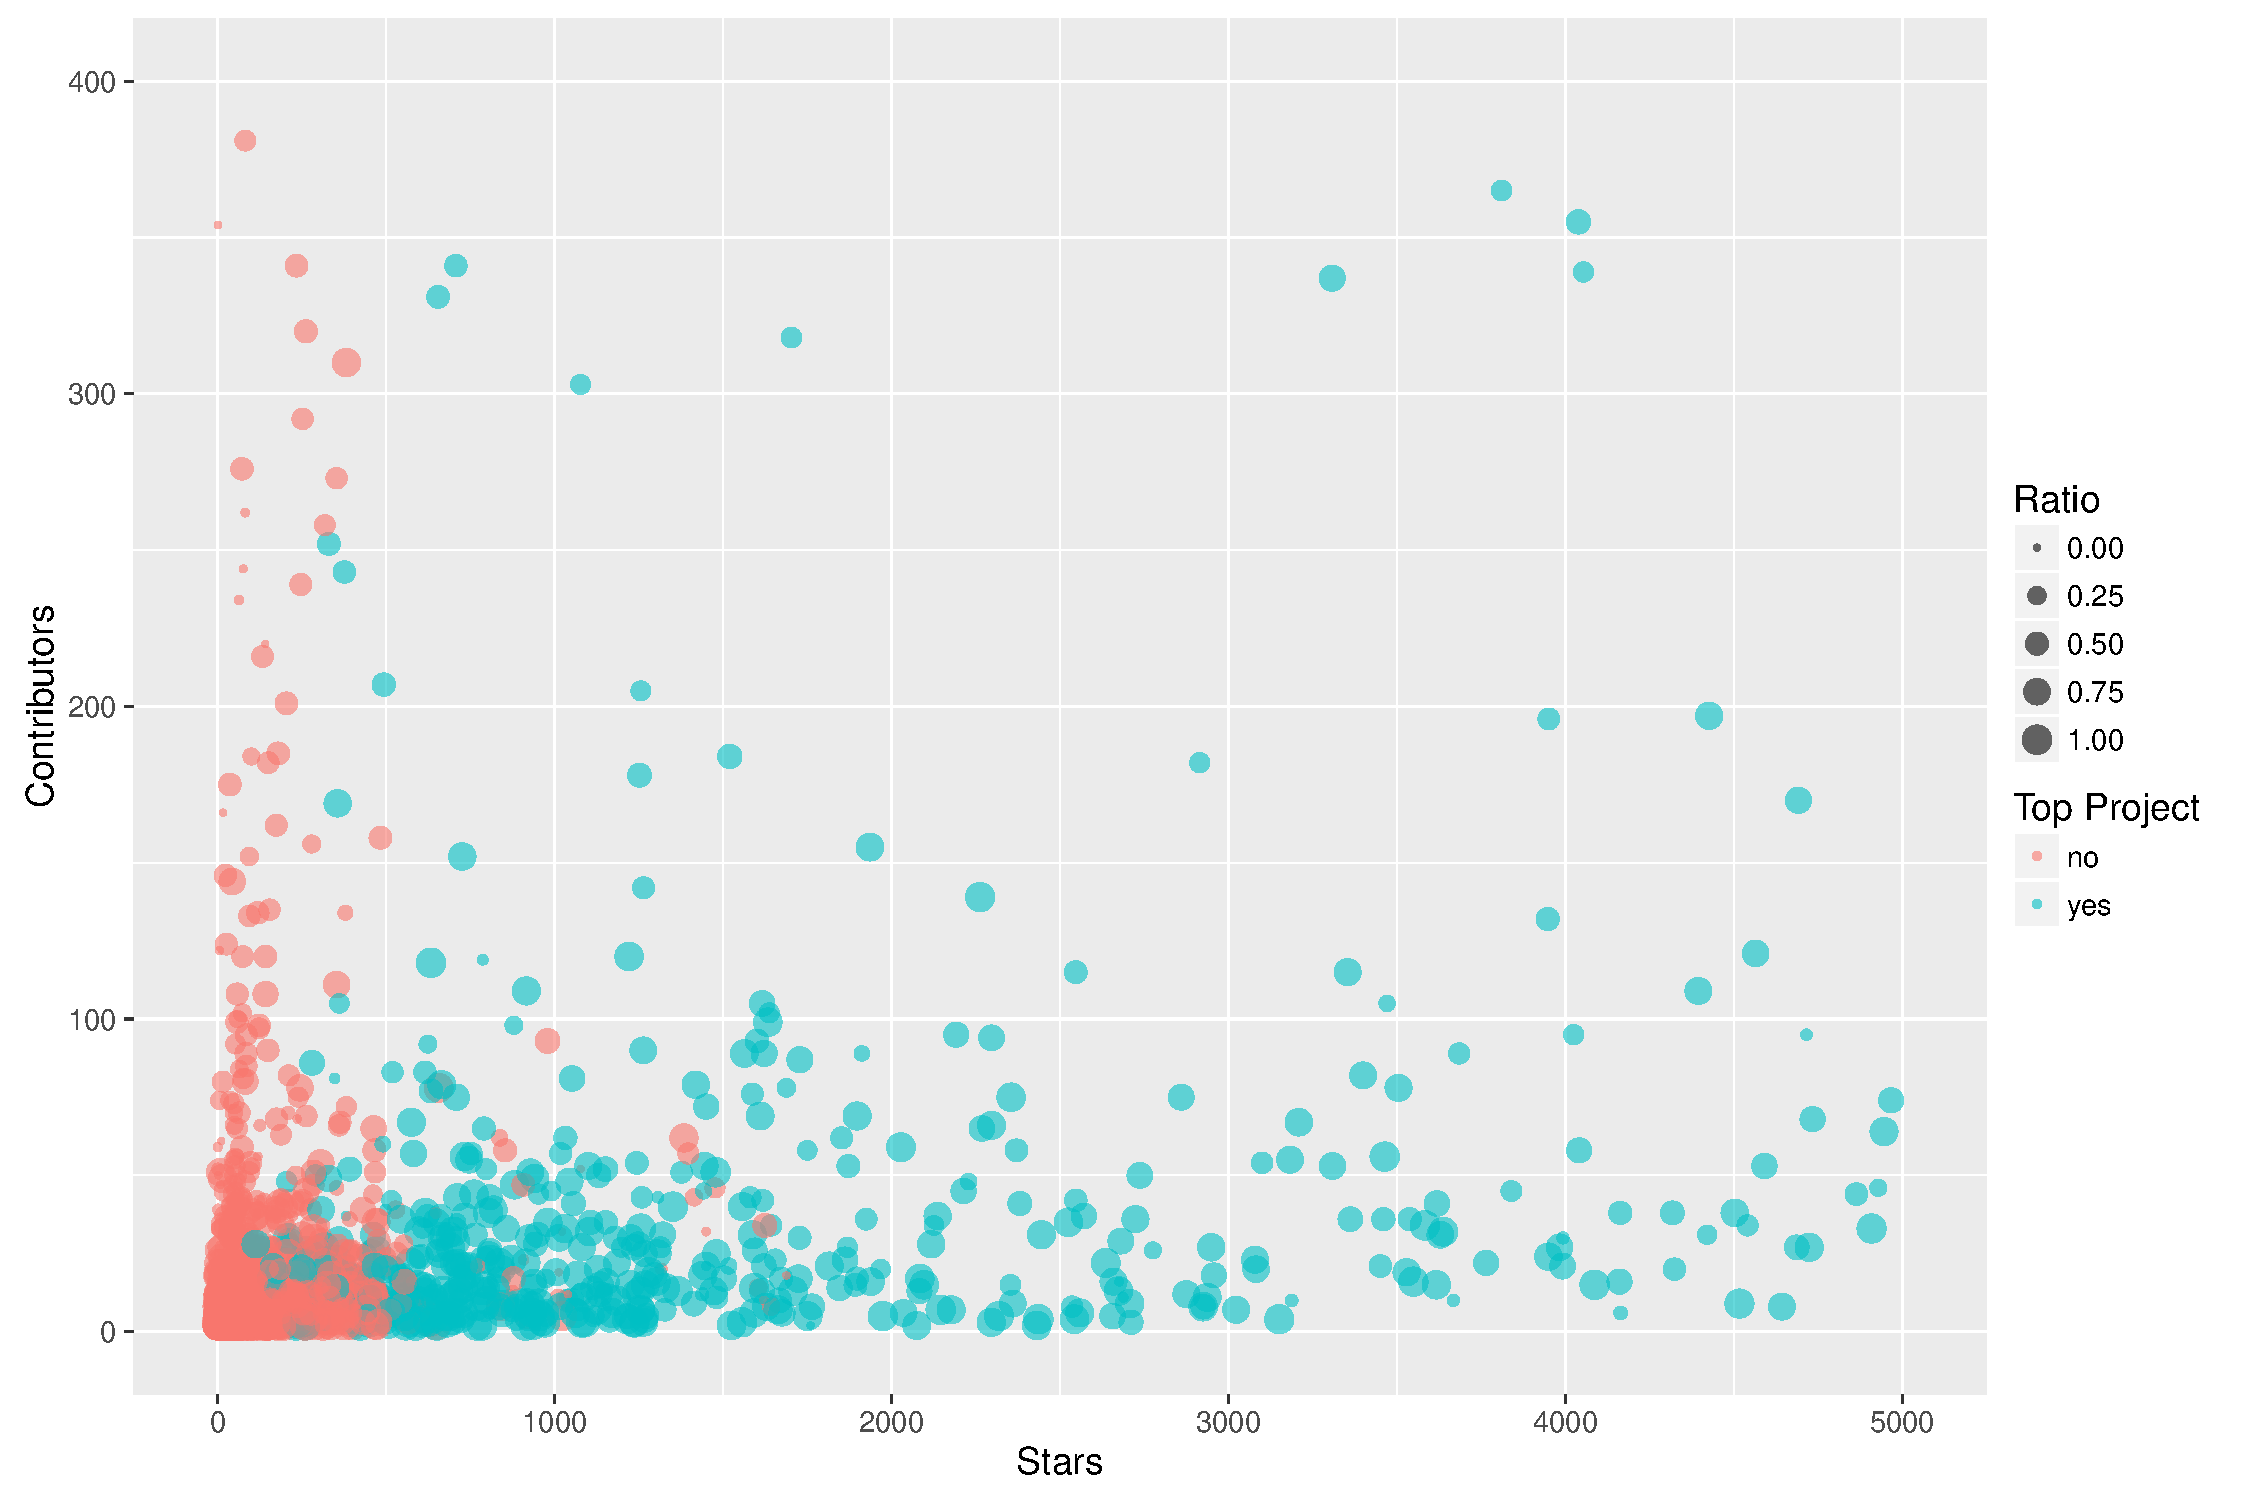
\includegraphics[page=1,scale=0.35]{../graphics/intro/stars_contributors.pdf}
	\caption{The "ratio" (code commitment share of firm employed developers), represented by size of dots, is quite high on all observed projects ($\geq 0.5$)}
\end{figure}

\begin{figure}[h]
	\centering
	\label{fig:stars_contributors_low_ratio_projects}
	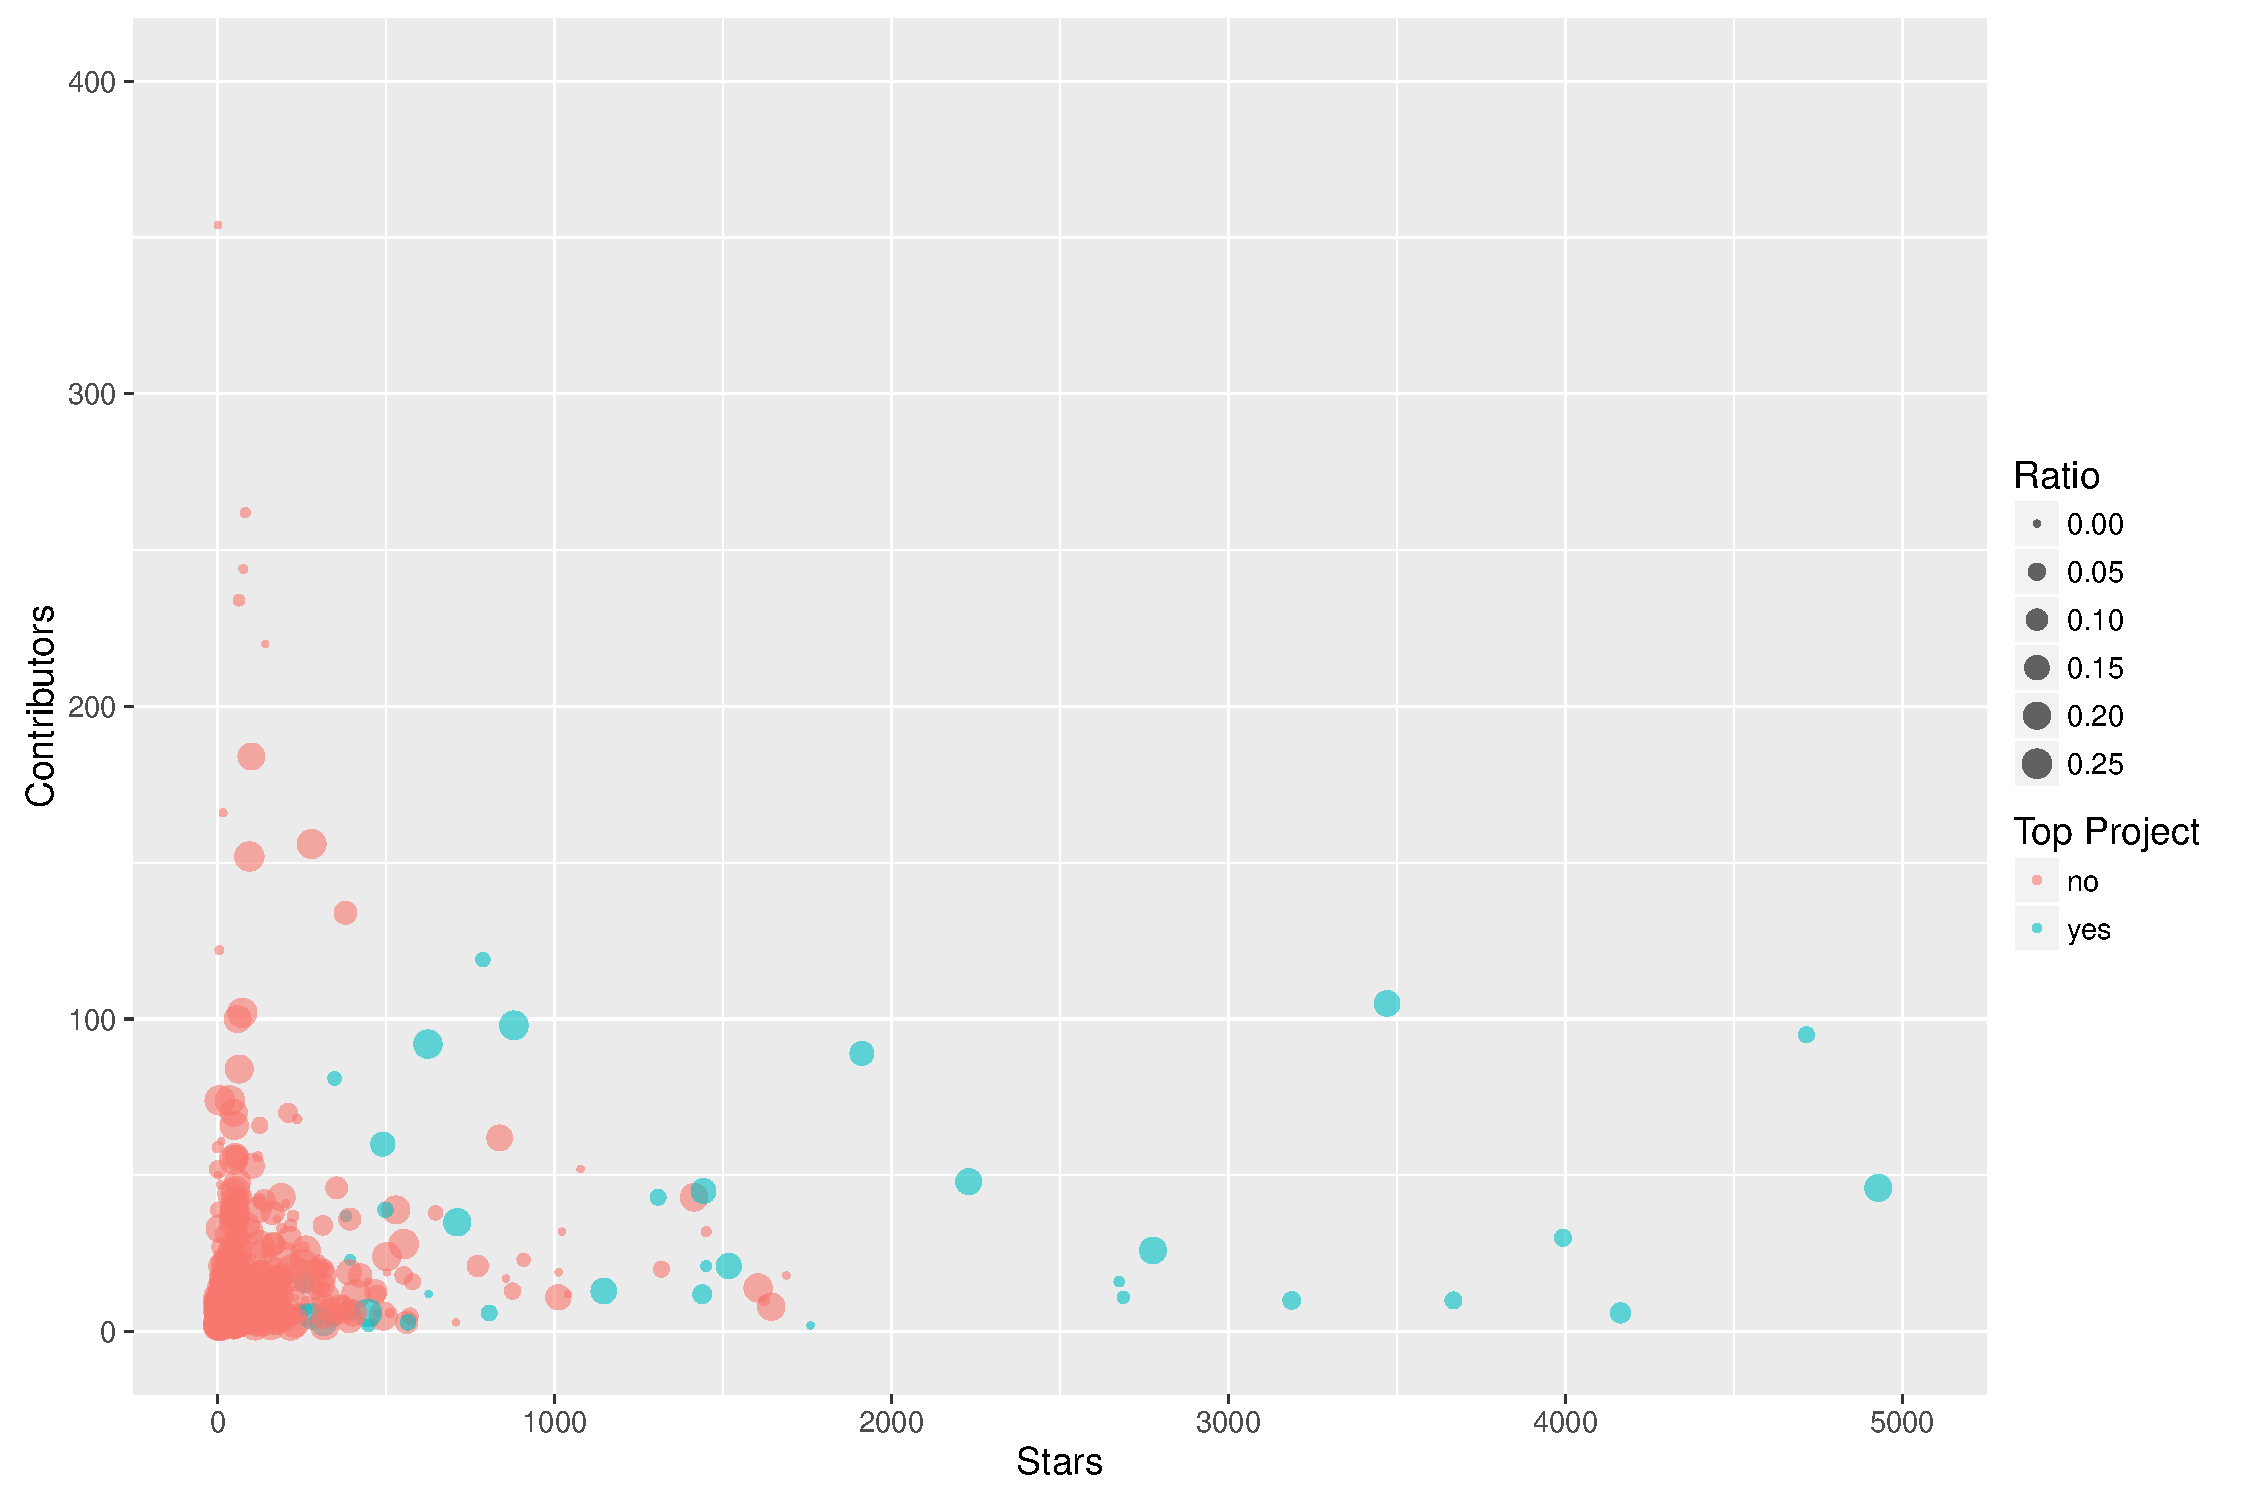
\includegraphics[page=1,scale=0.35]{../graphics/intro/stars_contributors_low_ratio_projects.pdf}
	\caption{If the ratio is low ($\leq 0.25$) there are fewer top projects / less stargazers}
\end{figure}

\begin{figure}
	\centering
	\label{fig:stars_contributors_high_ratio_projects}
	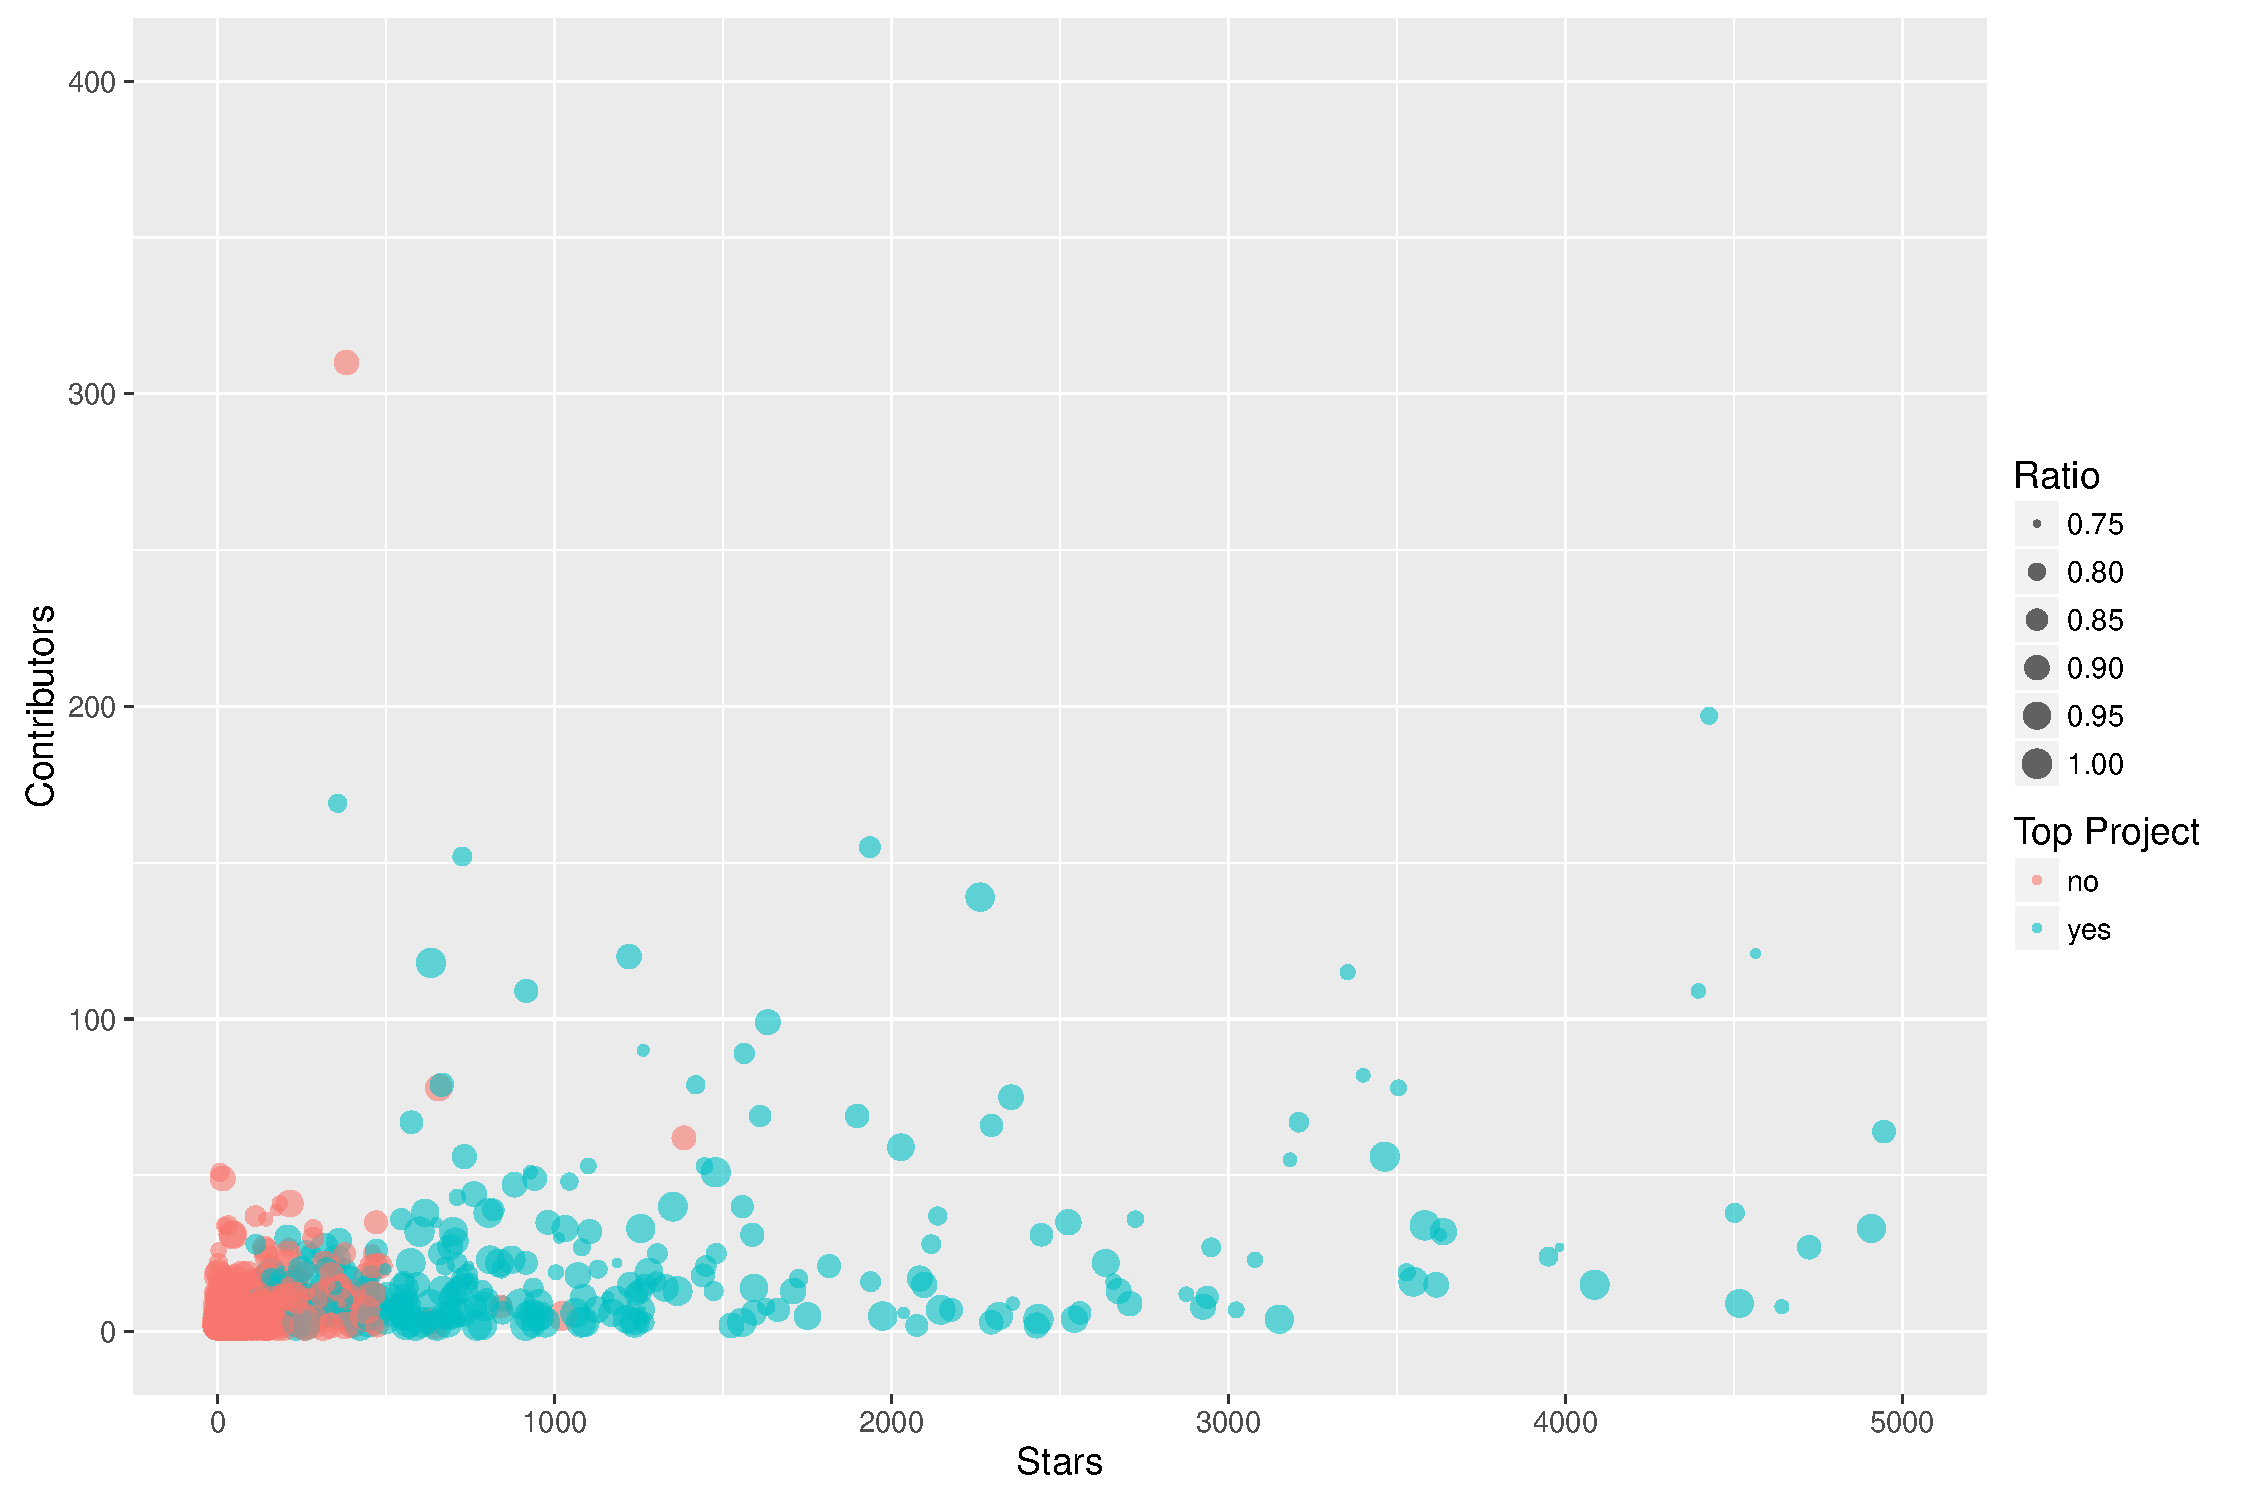
\includegraphics[page=1,scale=0.4]{../graphics/intro/stars_contributors_high_ratio_projects.pdf}
	\caption{If the ratio is higher ($\geq 0.75$) there are more top projects / stargazers}
\end{figure}

\begin{landscape}
\begin{figure}
	\centering
	\label{fig:code_contribution_age_ratio}
	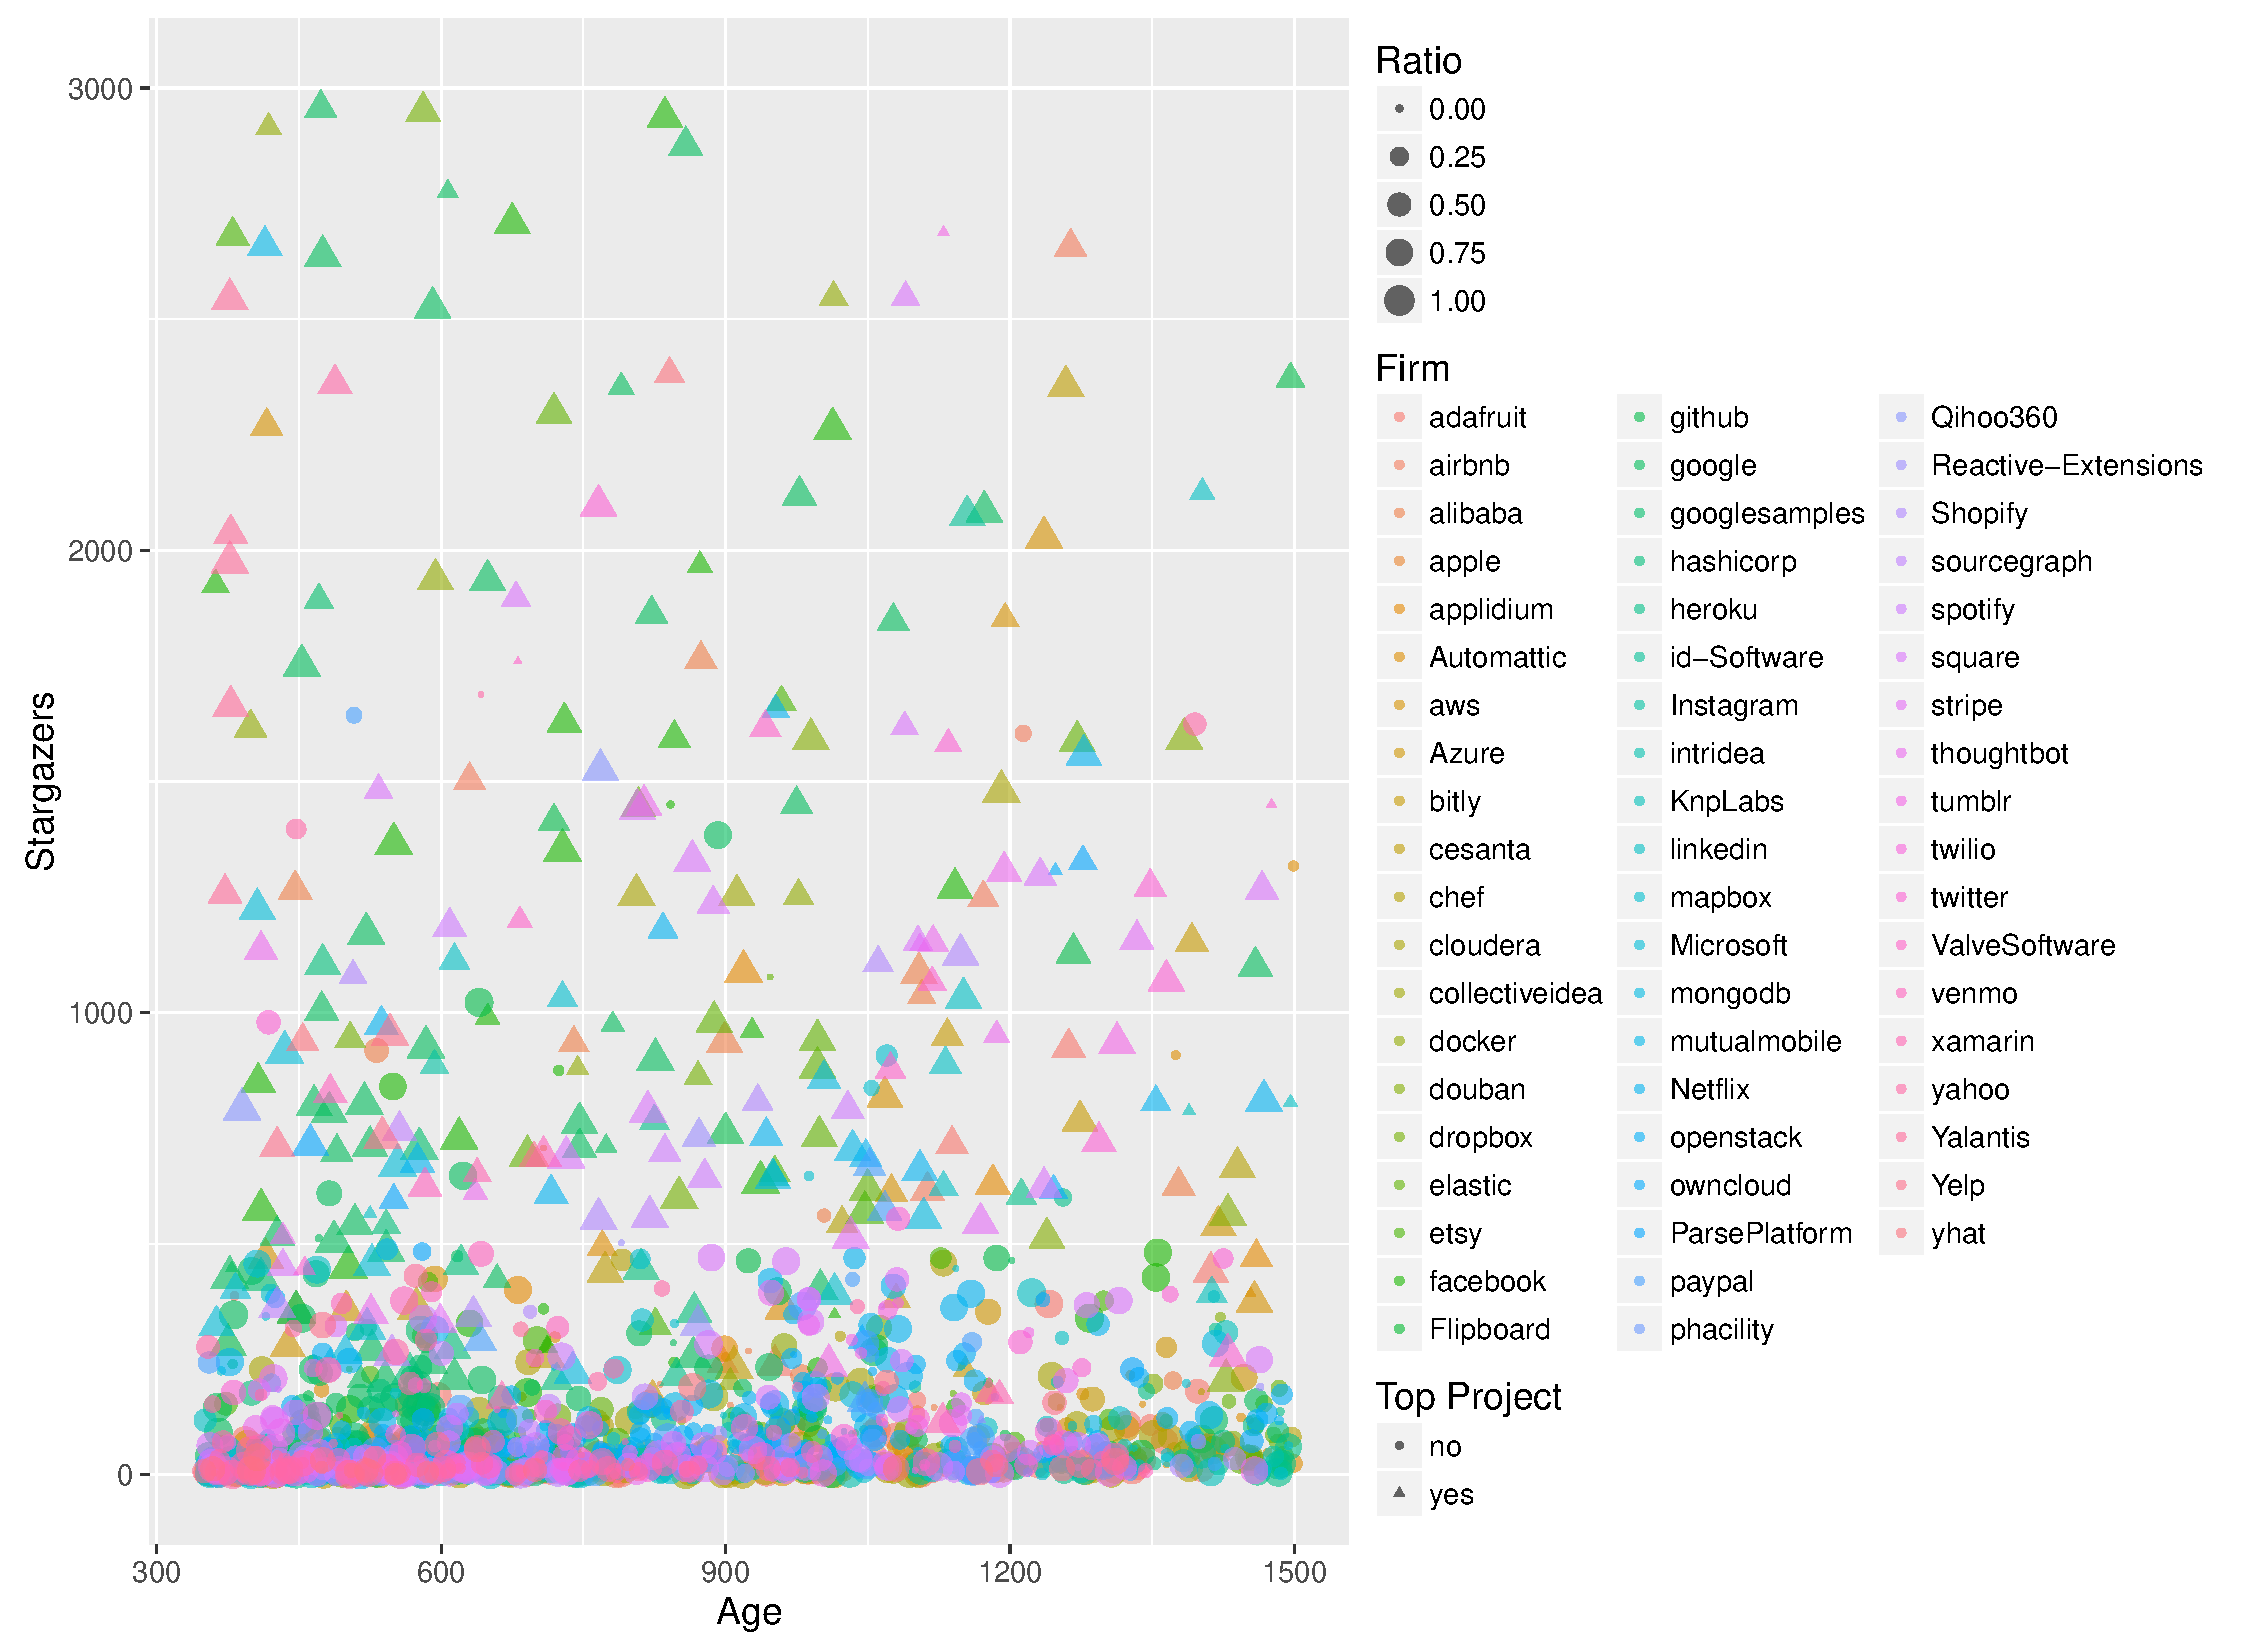
\includegraphics[page=1,scale=0.45]{../graphics/intro/code_contribution_age_ratio.pdf}
	\caption{The age of projects (in days), their popularity (number of stars), colored by firms, size of shapes by "ratio" (code commitment share of firm employed developers) and shape by "Top Project" or "Residual Project". All plotted projects are less than 4.5 years old.}
\end{figure}

\begin{figure}
	\centering
	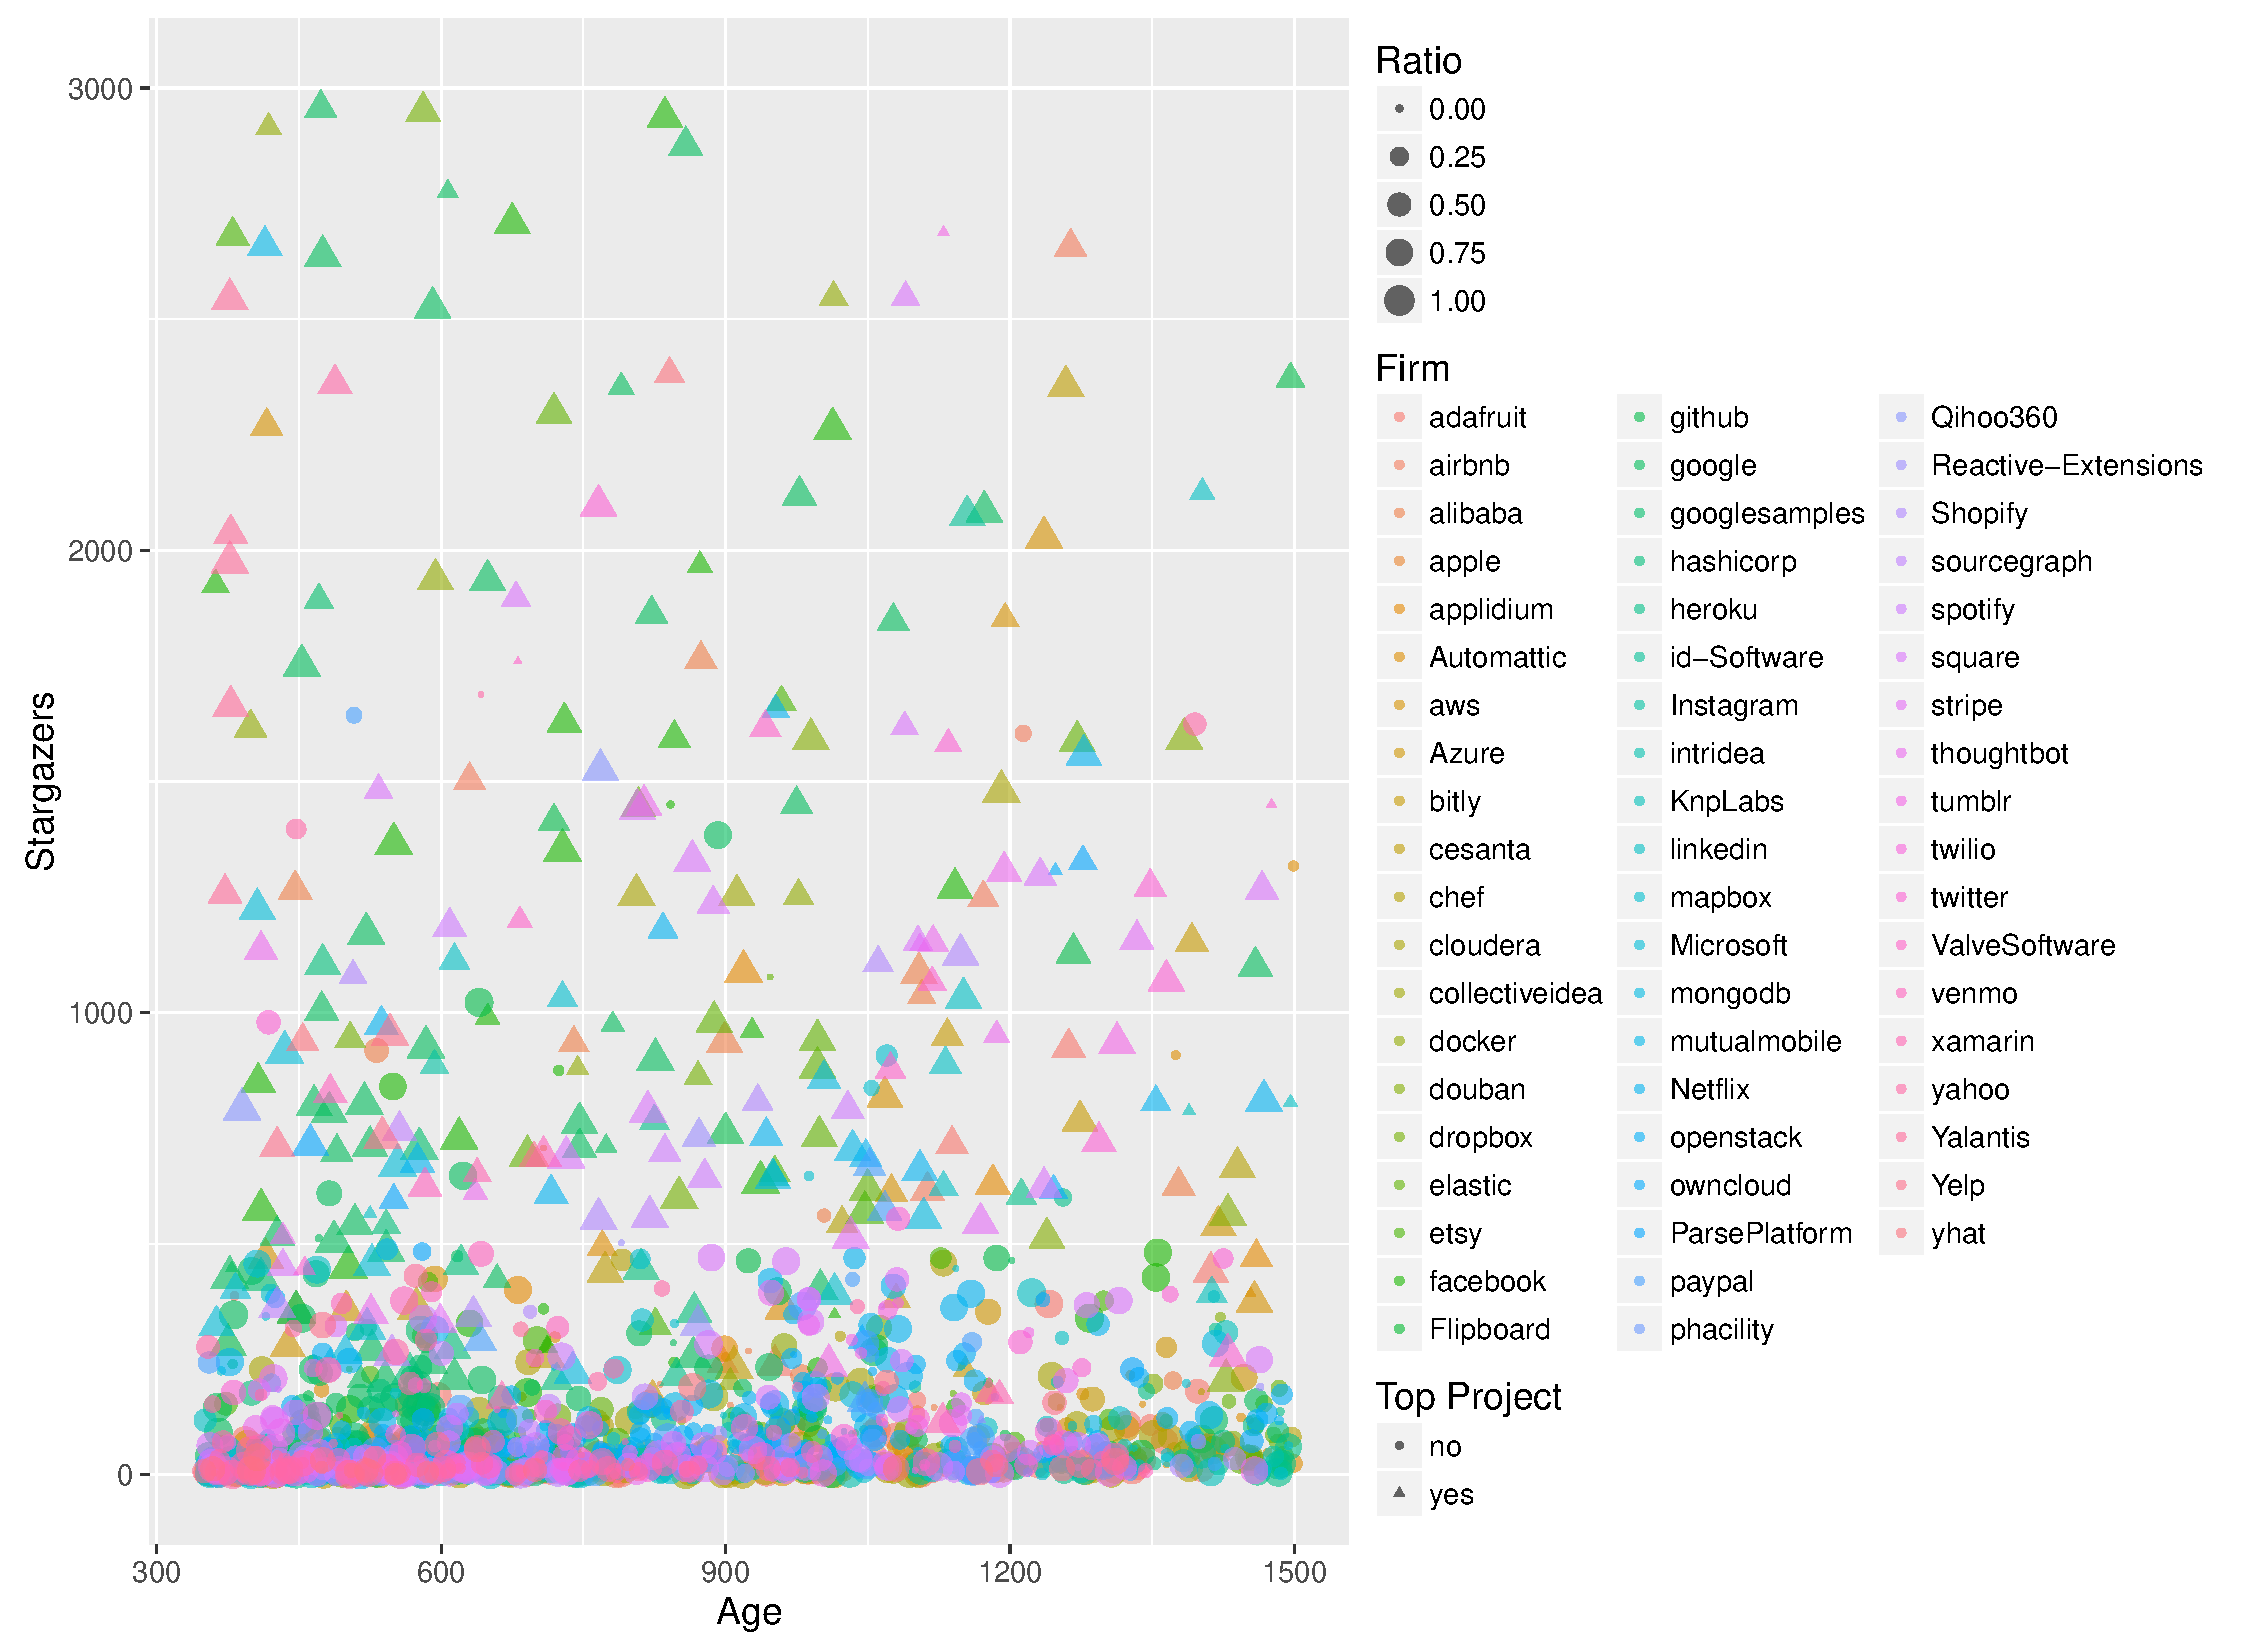
\includegraphics[page=1,scale=0.45]{../graphics/intro/code_contribution_age_ratio.pdf}
	\caption{The age of projects (in days), their popularity (number of stars), colored by (all) firms, size of shapes by "ratio" (code commitment share of firm employed developers) and shape by "Top Project" or "Residual Project". All plotted projects are less than 4.5 years old.}
	\label{fig:code_contribution_age_ratio}
\end{figure}

\begin{figure}
	\centering
	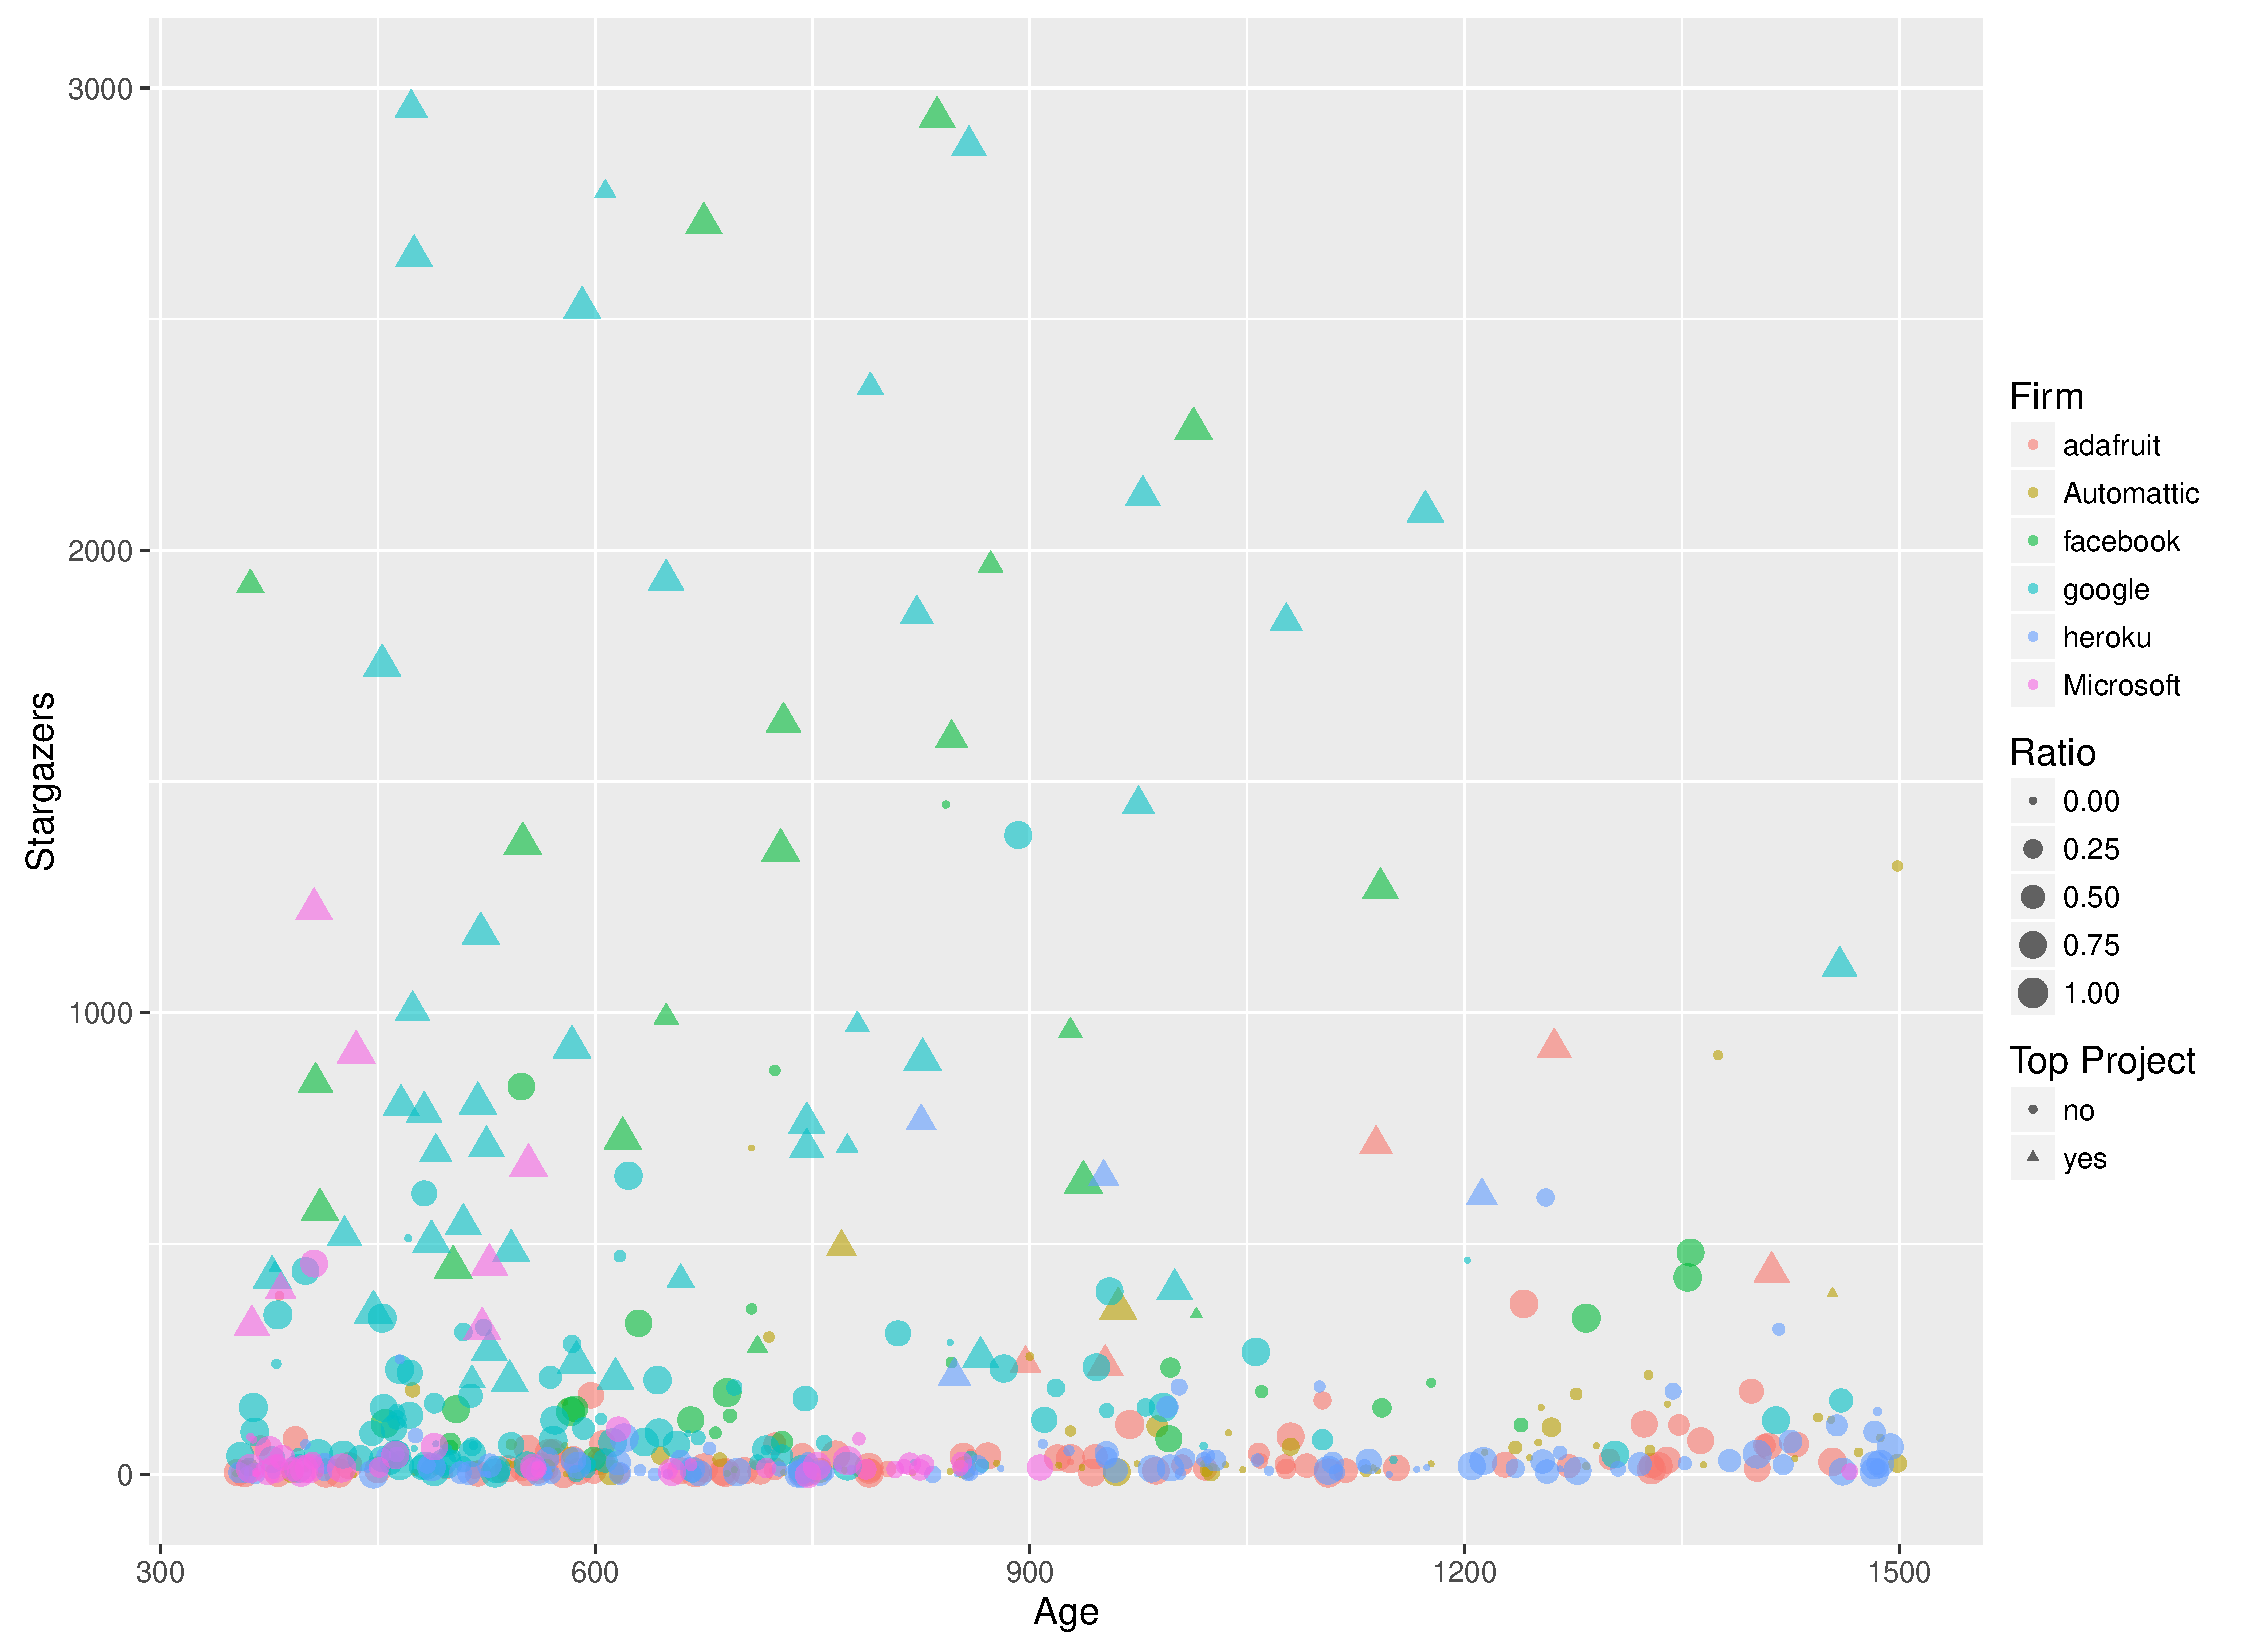
\includegraphics[page=1,scale=0.4]{../graphics/intro/code_contribution_age_firms_ratio.pdf}
	\caption{The age of projects (in days), their popularity (number of stars), colored by firms with most popular OS projects, size of shapes by "ratio" (code commitment share of firm employed developers) and shape by "Top Project" or "Residual Project". All plotted projects are less than 4.5 years old.}
	\label{fig:code_contribution_age_firms_ratio}
\end{figure}

\begin{figure}
	\centering
	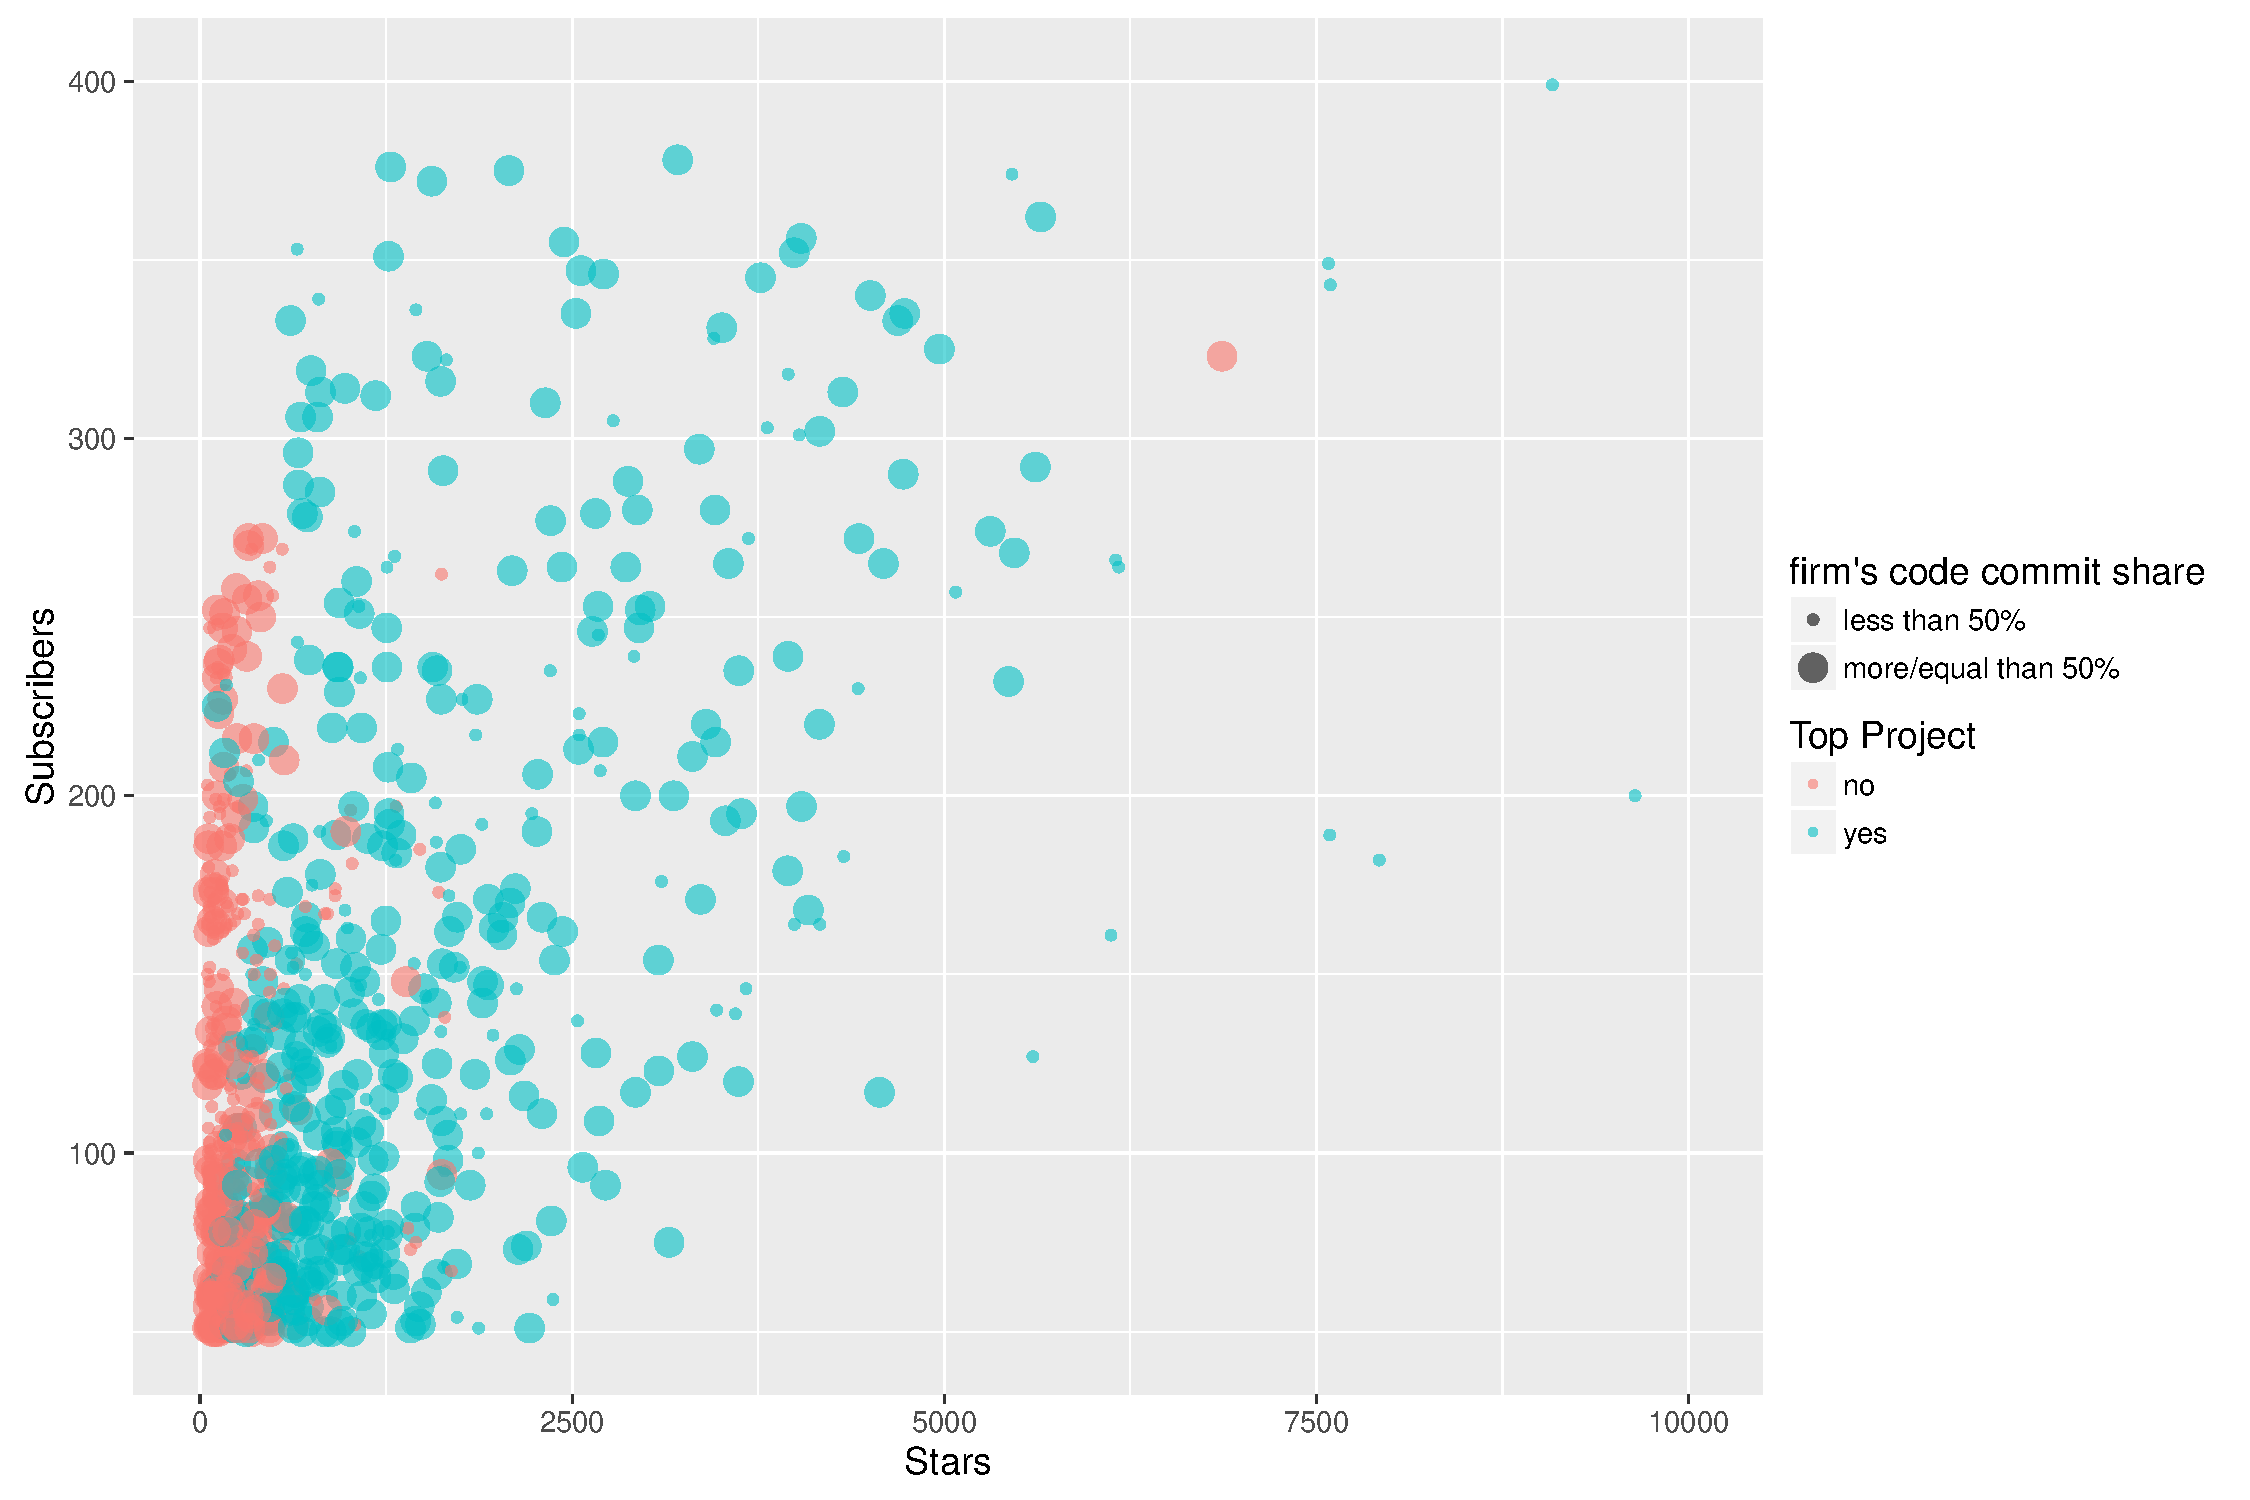
\includegraphics[page=1,scale=0.4]{../graphics/intro/stars_subscribers_ratio_top_10000.pdf}
	\caption{Seperation in ratio $< 0.5$ and $\geq 0.5$; Plotted with Stars against Subscribers (proxies for popularity), colored in Top and Residual Projects and scaled x-axis up to 10,000 stars.}
	\label{fig:stars_subscribers_ratio_top_10000}
\end{figure}

\begin{figure}
	\centering
	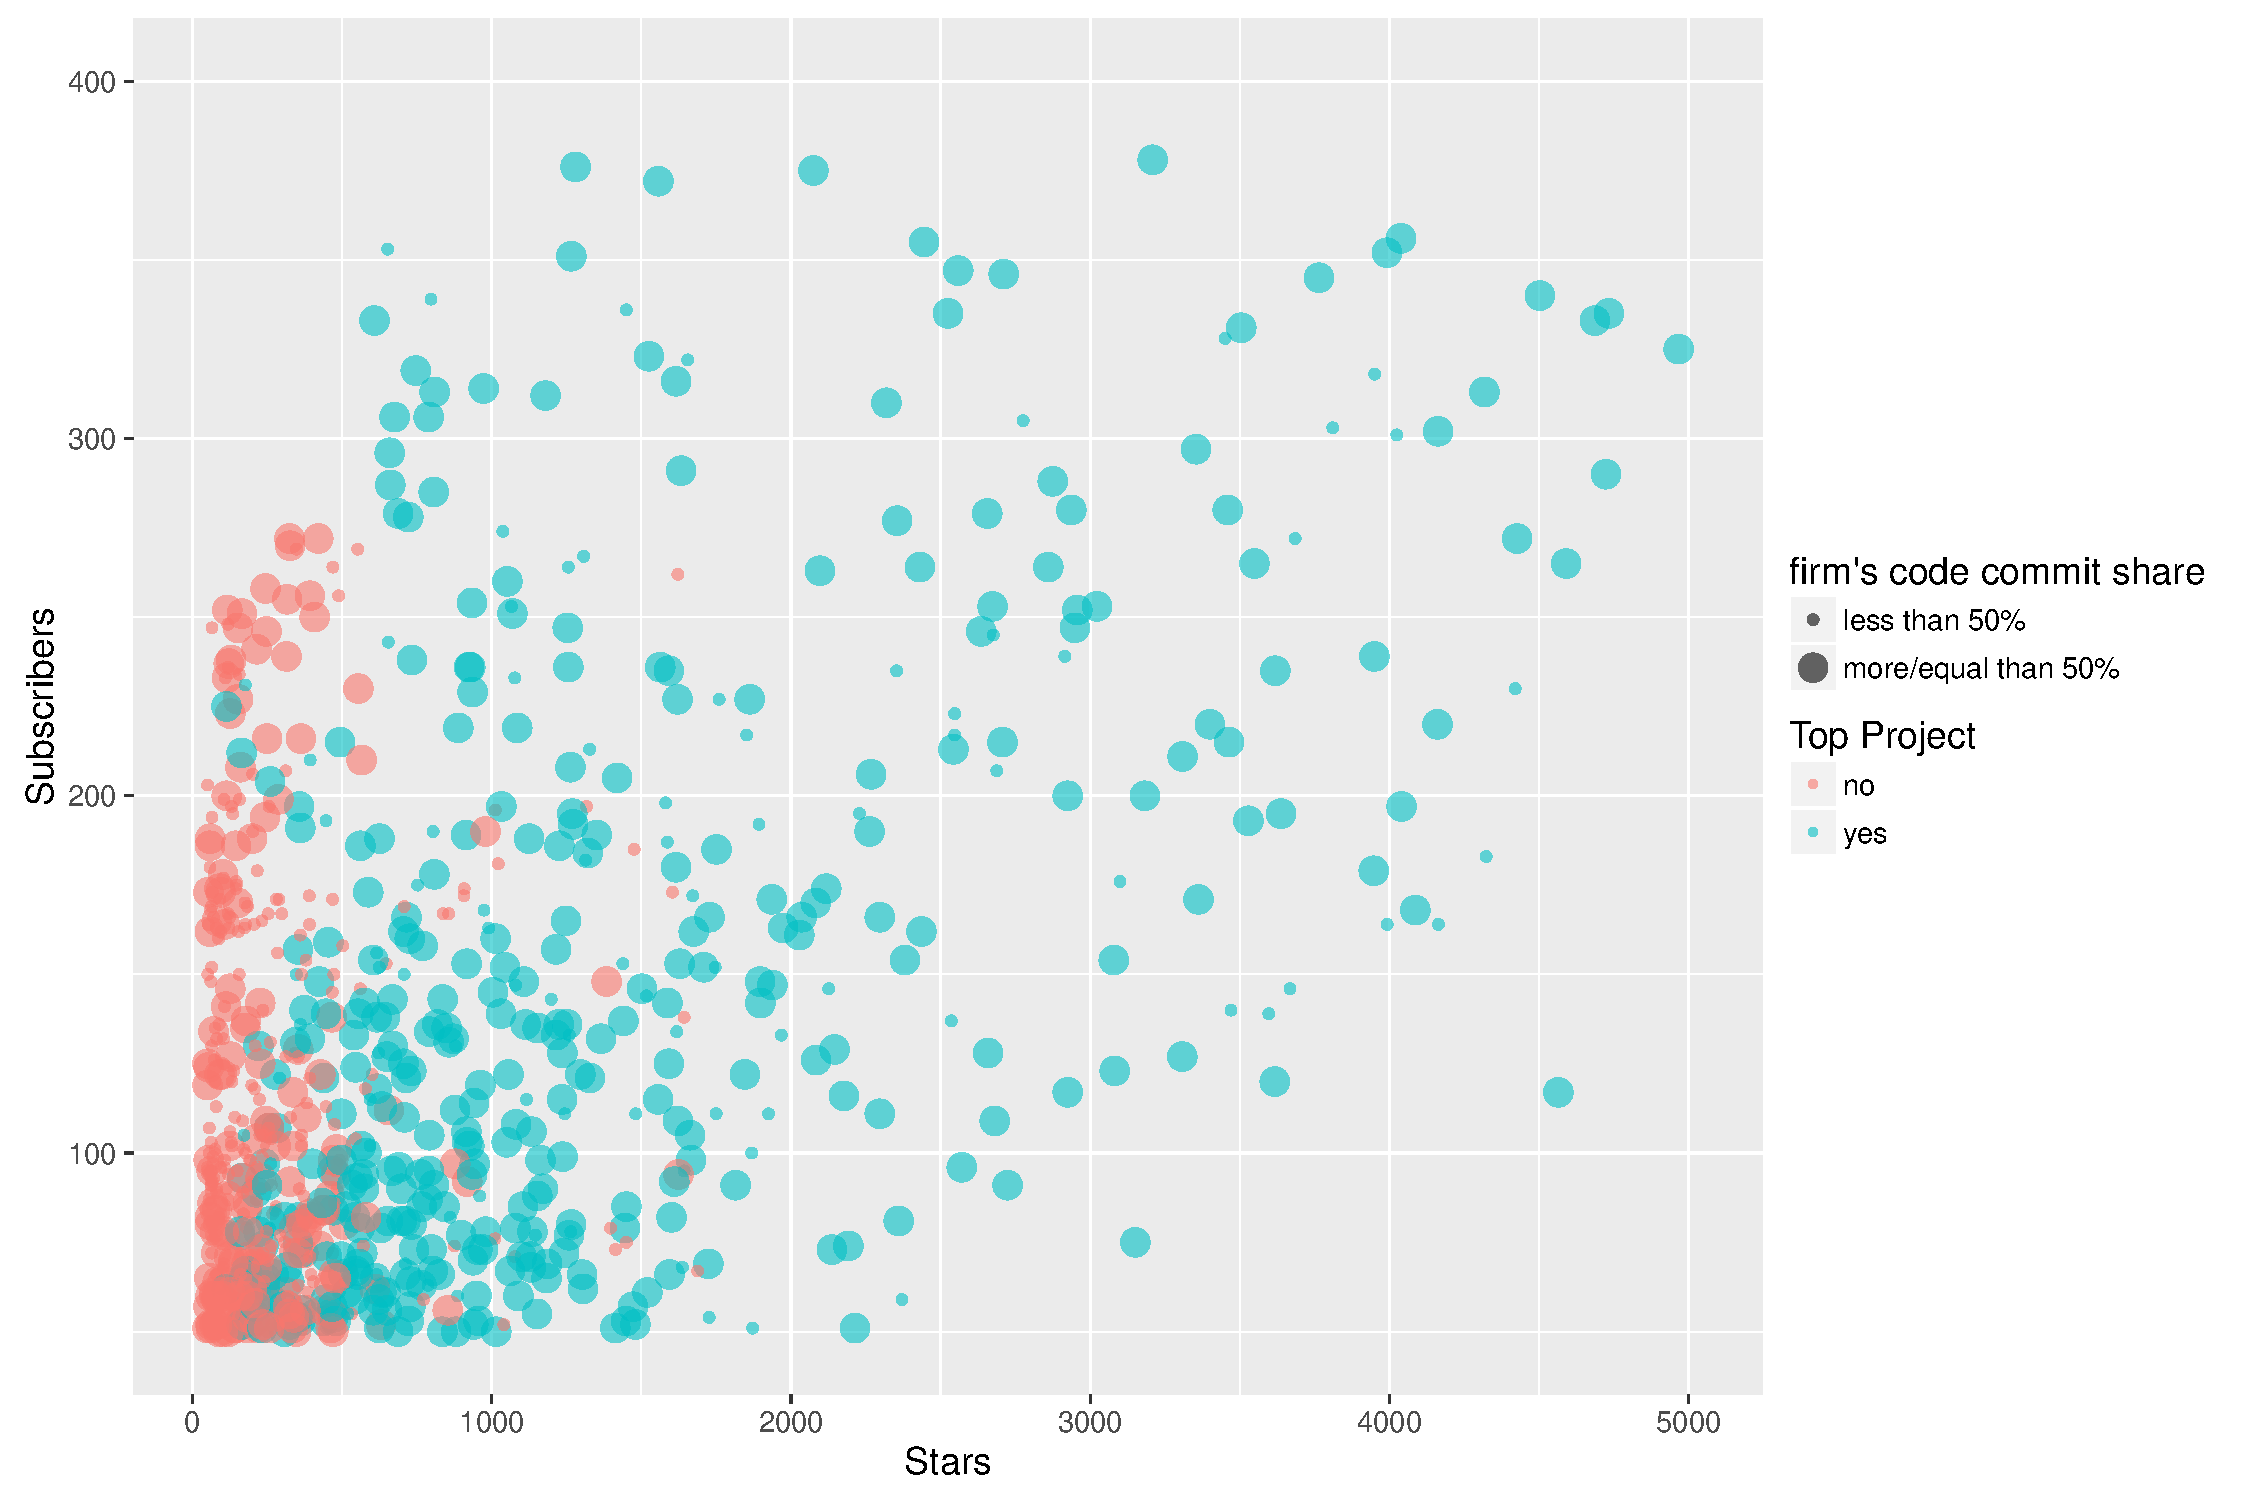
\includegraphics[page=1,scale=0.4]{../graphics/intro/stars_subscribers_ratio_top_5000.pdf}
	\caption{Same as figure \ref{fig:stars_subscribers_ratio_top_10000} but with scaled x-axis up to 5000 stars.}
	\label{fig:stars_subscribers_ratio_top_5000}
\end{figure}

\begin{figure}
	\centering
	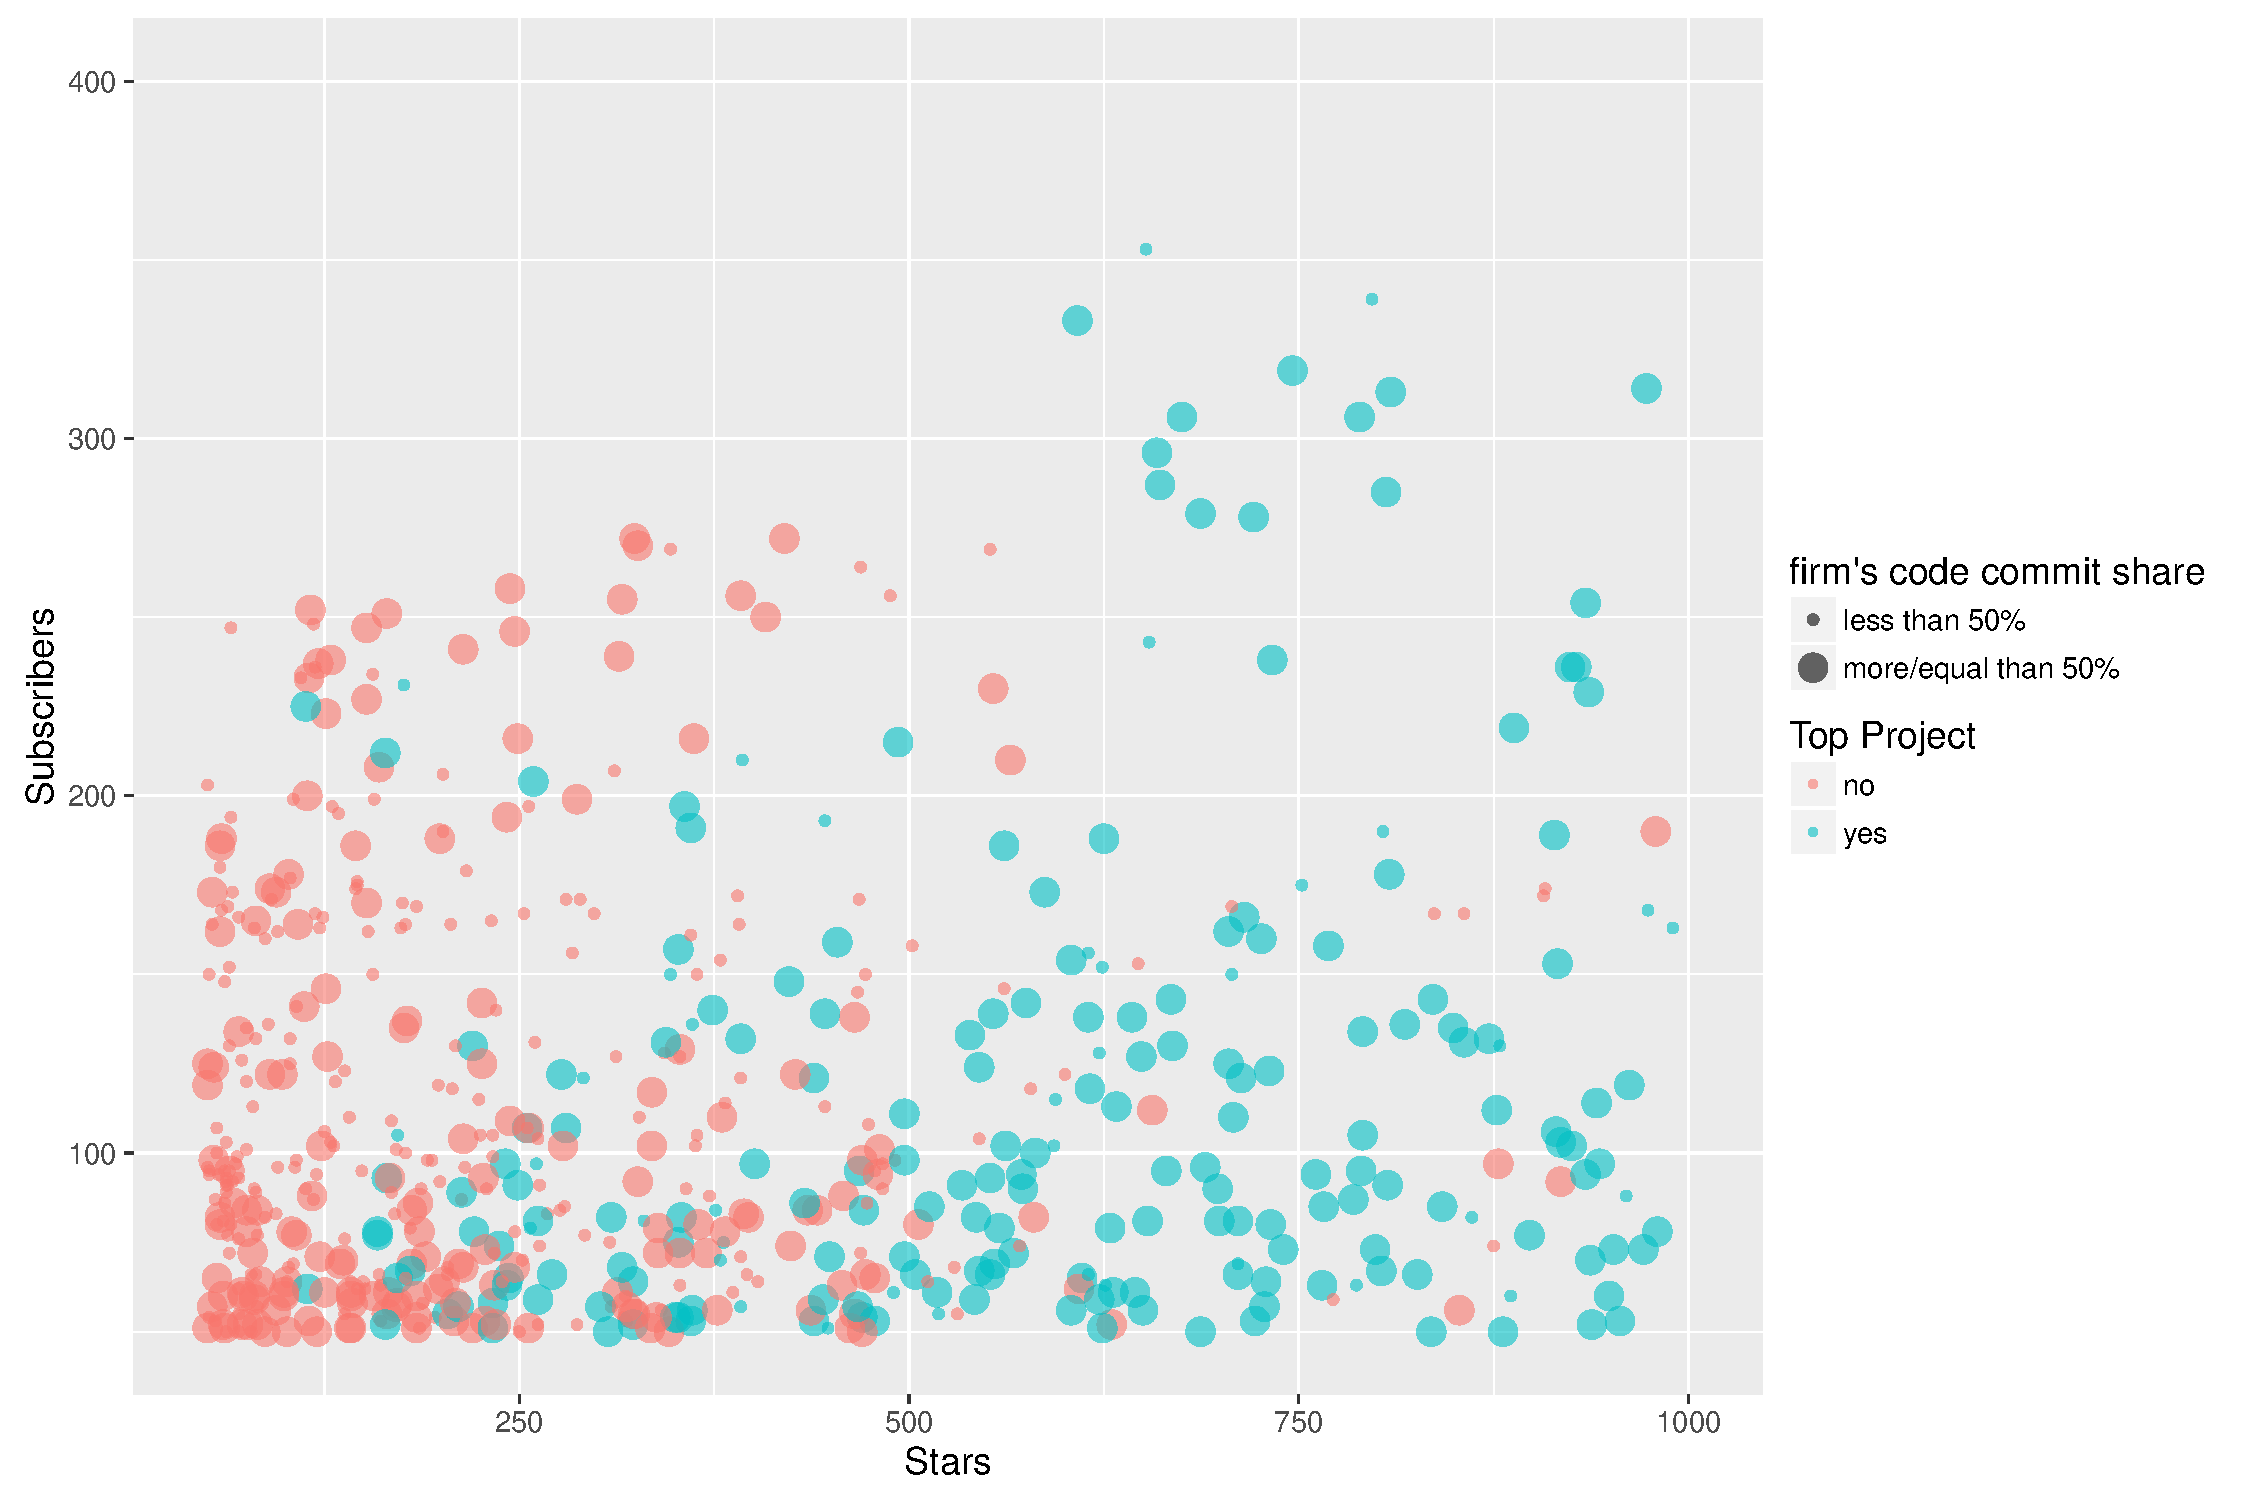
\includegraphics[page=1,scale=0.4]{../graphics/intro/stars_subscribers_ratio_top_1000.pdf}
	\caption{Same as figure \ref{fig:stars_subscribers_ratio_top_10000} but with scaled x-axis up to 1000 stars.}
	\label{fig:stars_subscribers_ratio_top_1000}
\end{figure}

\end{landscape}







\subsection{Plots for H 1.1}
\label{sec:h_1.1_plots}

See page \pageref{sec:lm_plots_description} for explanation of slopes and axes.

\vspace{20 pt}

\begin{minipage}{.5\textwidth}
	\centering
	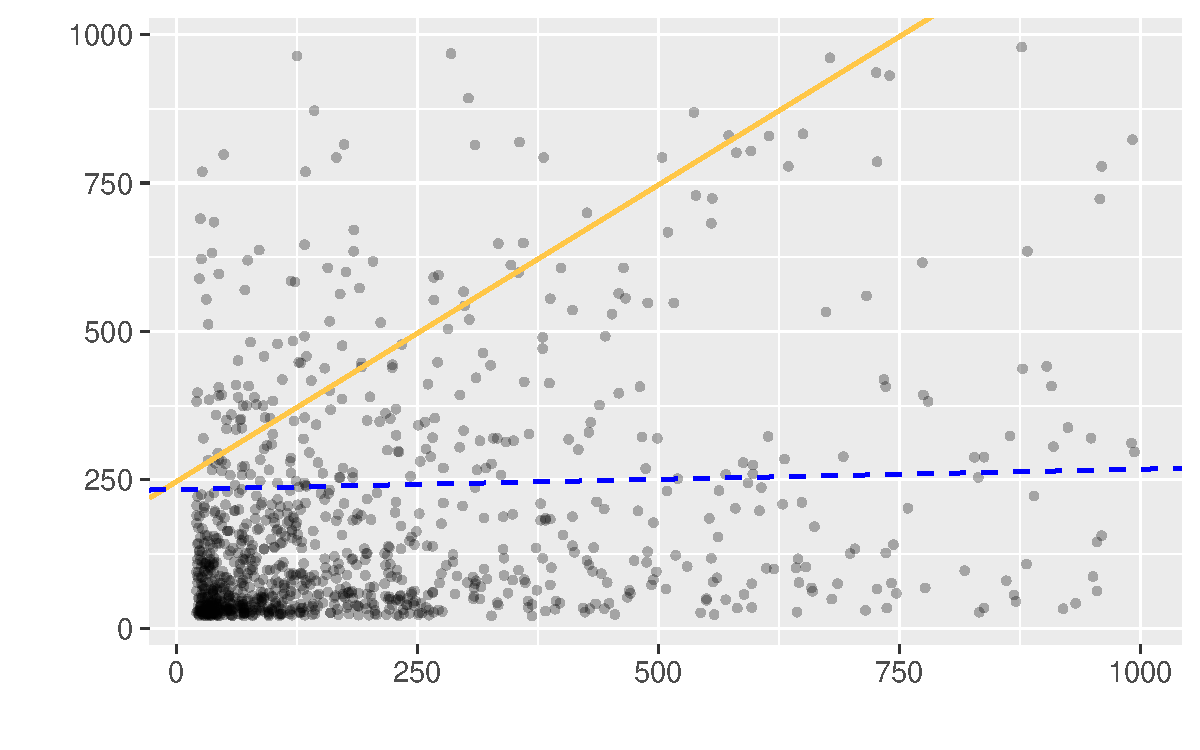
\includegraphics[page=1,scale=0.3]{../hypotheses/lm_in_ext_model_1_2.pdf}
  \captionof{figure}{All Projects (Model 1.1.1 - 1.1.2)}
  \label{fig:hyp1_model_1-2}
\end{minipage}
\begin{minipage}{.5\textwidth}
	\centering
	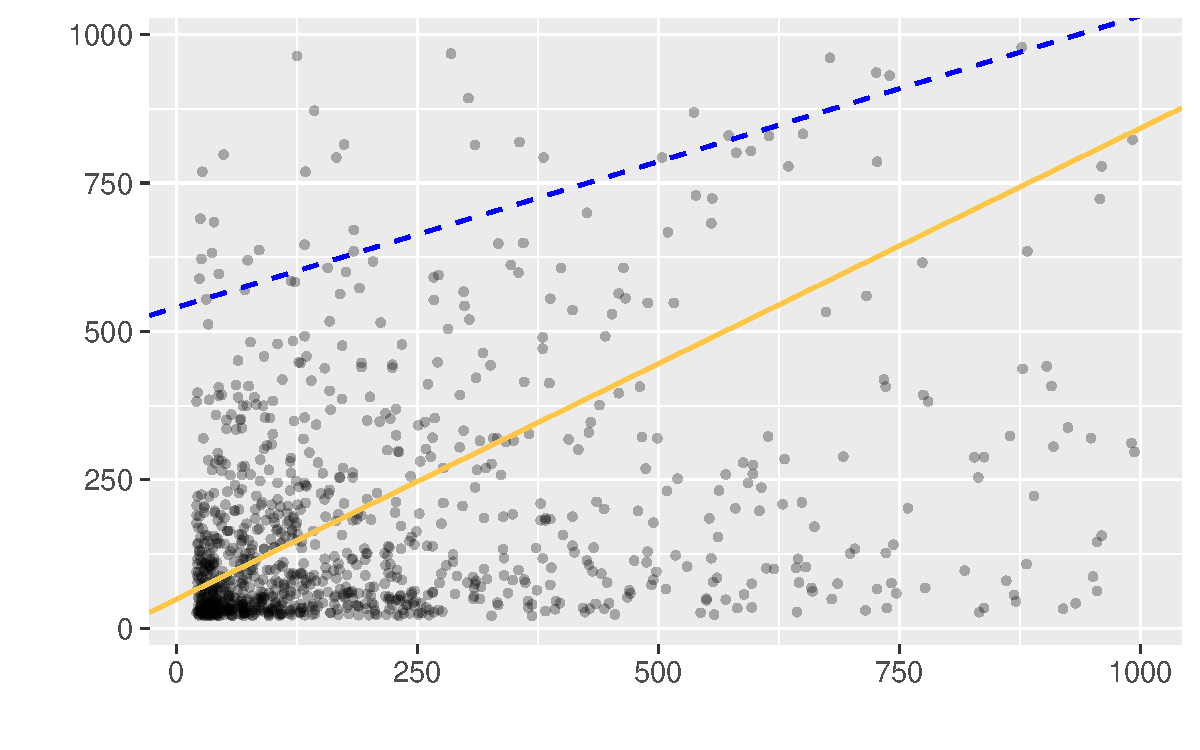
\includegraphics[page=1,scale=0.3]{../hypotheses/lm_in_ext_model_3_4.pdf}
  \captionof{figure}{Top Projects (Model 1.1.3 - 1.1.4)}
  \label{fig:hyp1_model_3-4}
\end{minipage}

\vspace{20 pt}

\begin{minipage}{.5\textwidth}
	\centering
	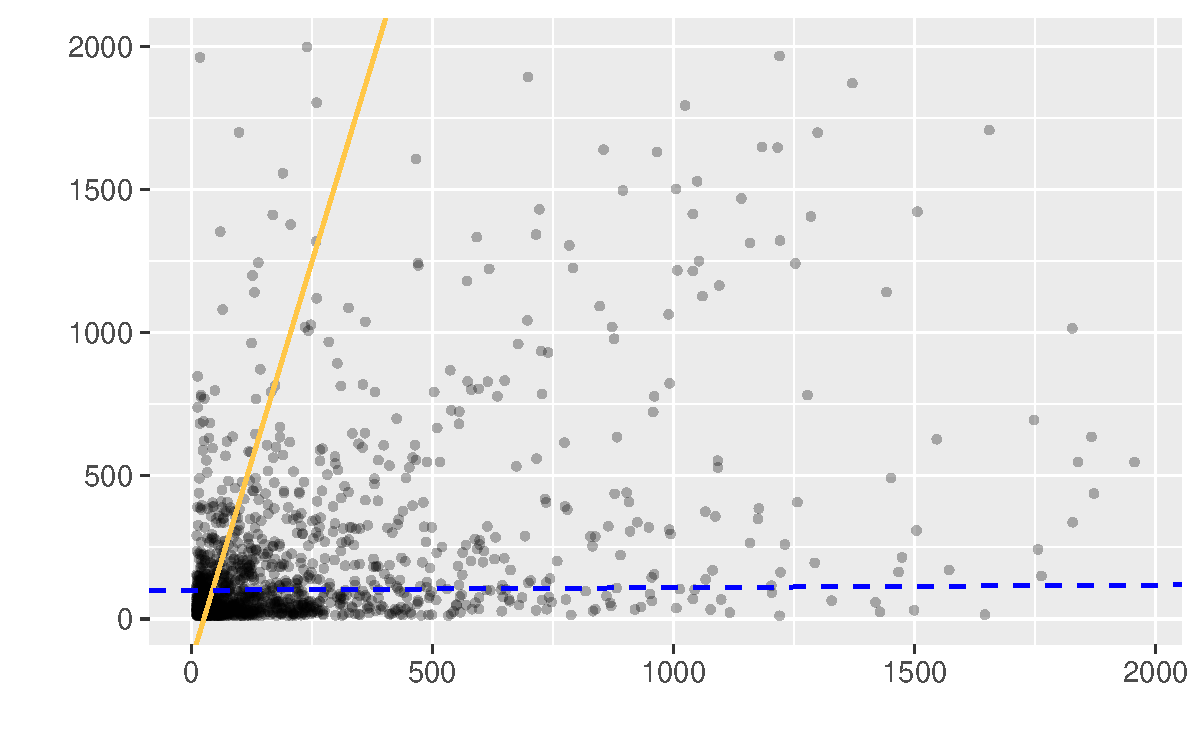
\includegraphics[page=1,scale=0.3]{../hypotheses/lm_in_ext_model_5_6.pdf}
  \captionof{figure}{Residual Projects (Model 1.1.5 - 1.1.6)}
  \label{fig:hyp1_model_5-6}
\end{minipage}
\begin{minipage}{.5\textwidth}
	\centering
	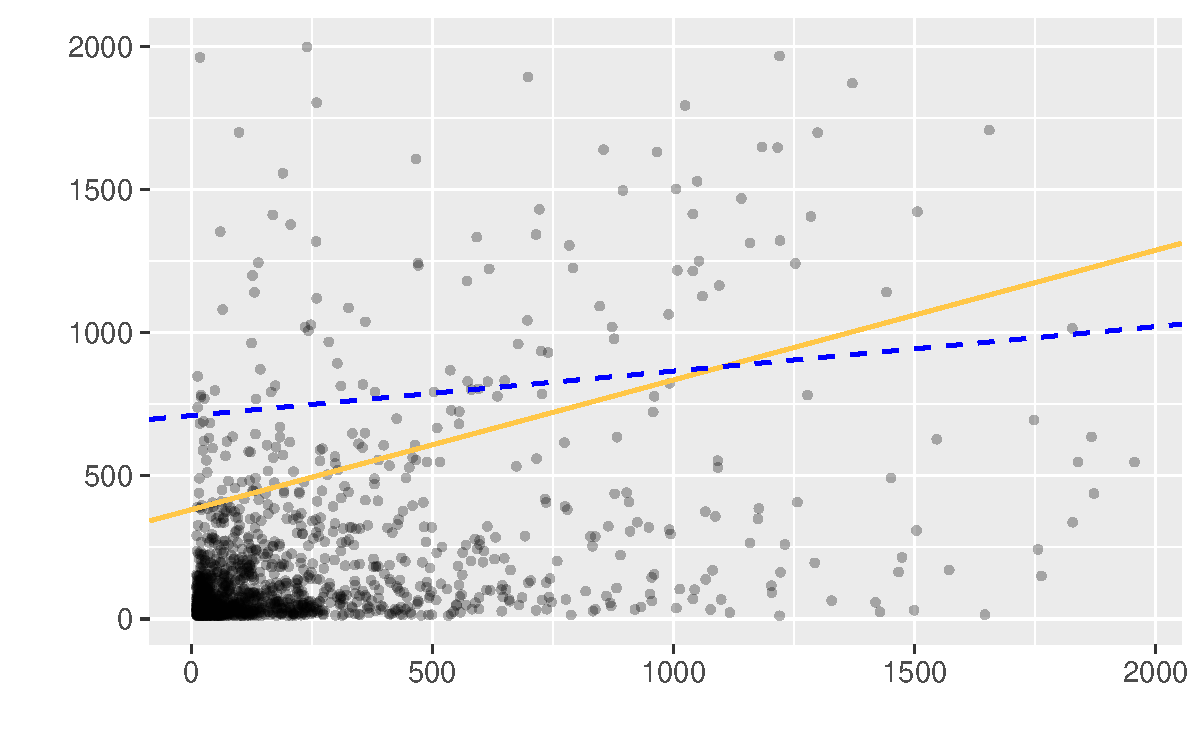
\includegraphics[page=1,scale=0.3]{../hypotheses/lm_in_ext_model_7_8.pdf}
  \captionof{figure}{Older Top Projects (Model 1.1.7 - 1.1.8)}
  \label{fig:hyp1_model_7-8}
\end{minipage}

\vspace{20 pt}

\begin{minipage}{.5\textwidth}
	\centering
	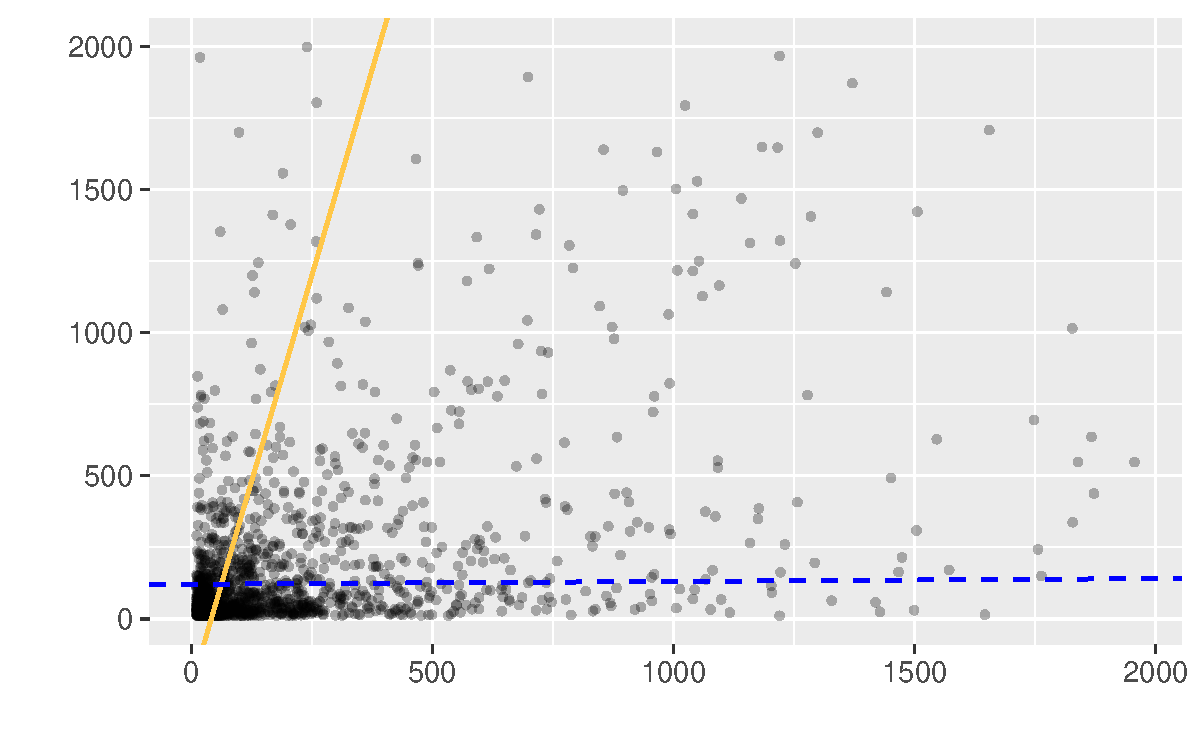
\includegraphics[page=1,scale=0.3]{../hypotheses/lm_in_ext_model_9_10.pdf}
  \captionof{figure}{Older Residual Projects (Model 1.1.9  - 1.1.10)}
  \label{fig:hyp1_model_9-10}
\end{minipage}
\begin{minipage}{.5\textwidth}
	\centering
	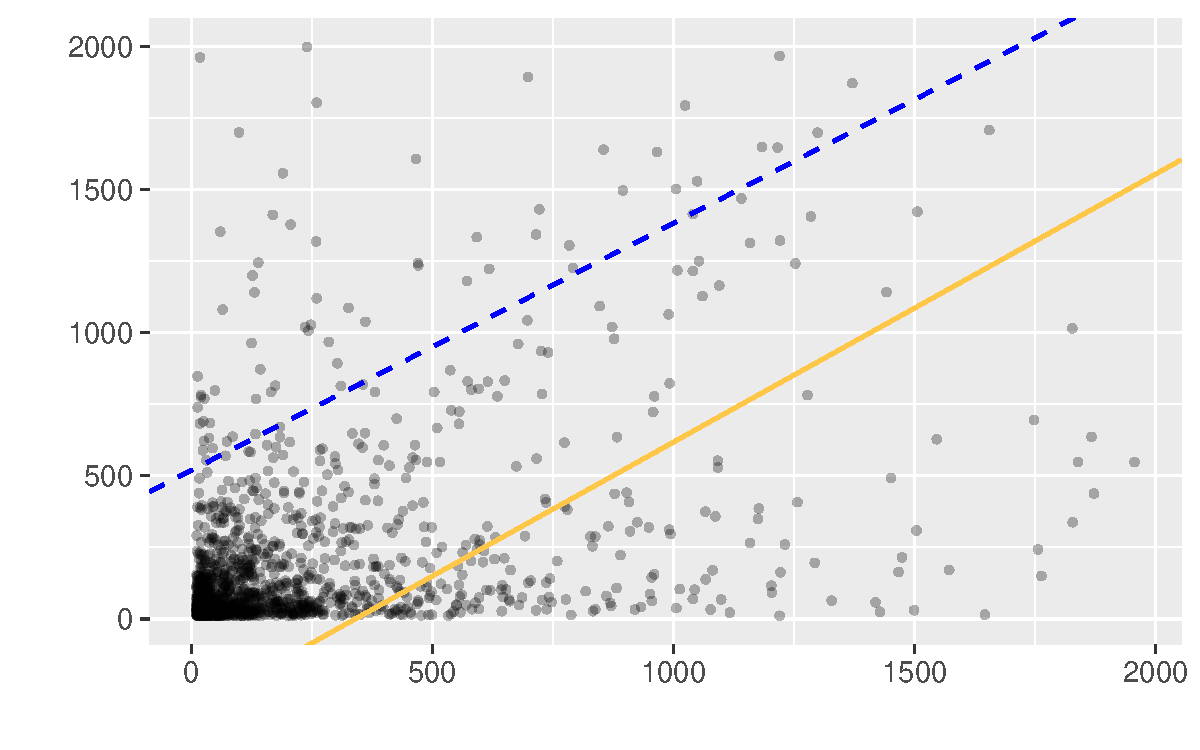
\includegraphics[page=1,scale=0.3]{../hypotheses/lm_in_ext_model_11_12.pdf}
  \captionof{figure}{Younger Top Projects (Model 1.1.11 - 1.1.12)}
  \label{fig:hyp1_model_11-12}
\end{minipage}





\subsection{Plots for H 1.2.1}
\label{sec:h_1.2.1_plots}

See page \pageref{sec:lm_plots_description} for explanation of slopes and axes.

\vspace{20 pt}

\begin{minipage}{.5\textwidth}
	\centering
	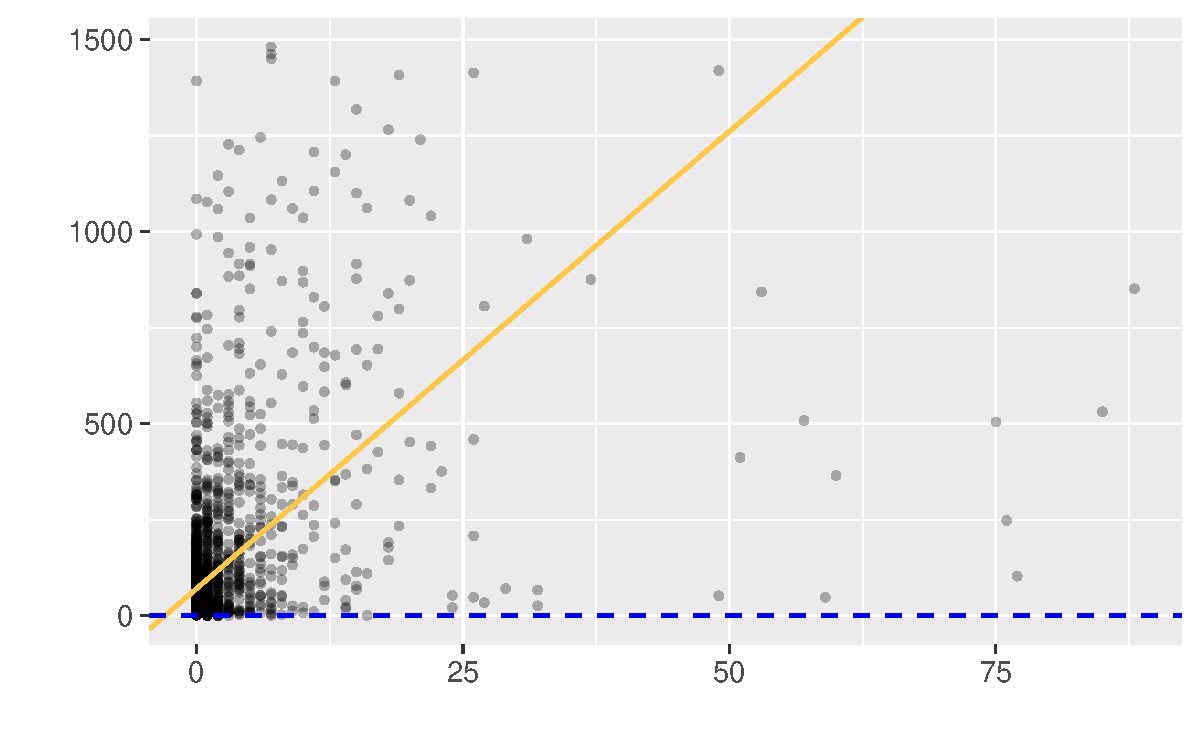
\includegraphics[page=1,scale=0.3]{../hypotheses/lm_issues_model_1_2.pdf}
  \captionof{figure}{All Projects (Model 1.2.1 - 1.2.2)}
  \label{fig:hyp1_issue_model_1-2}
\end{minipage}
\begin{minipage}{.5\textwidth}
	\centering
	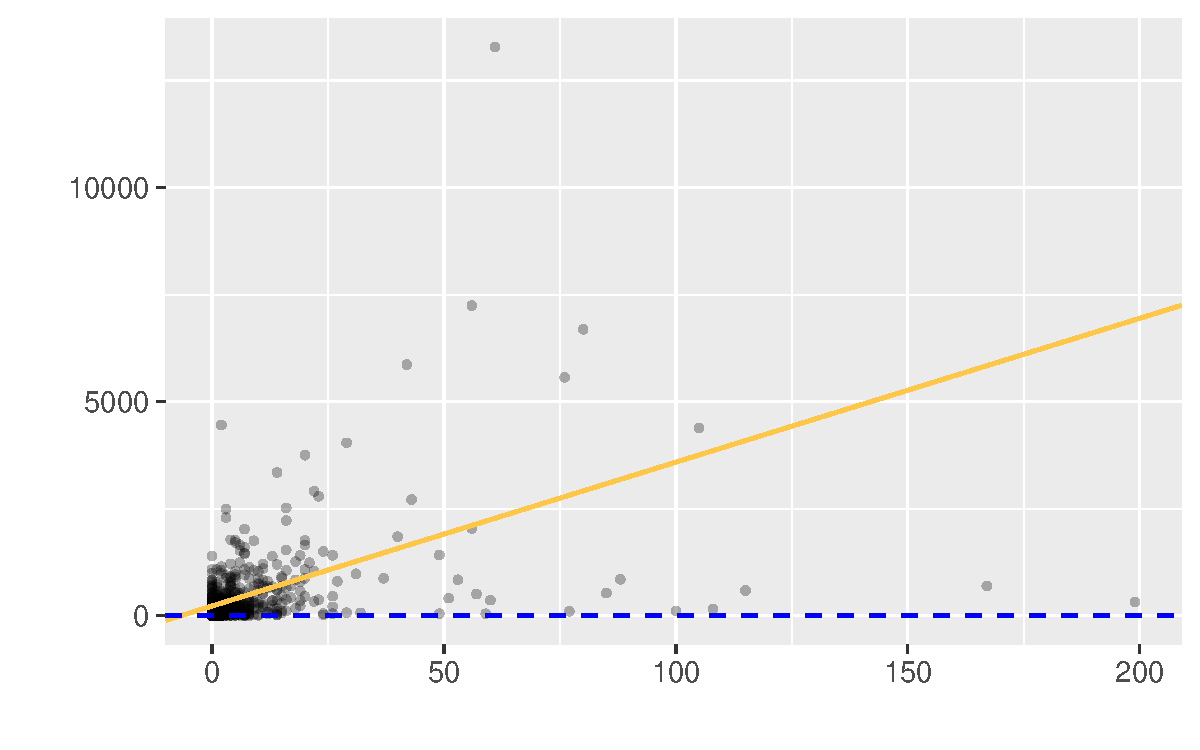
\includegraphics[page=1,scale=0.3]{../hypotheses/lm_issues_model_3_4.pdf}
  \captionof{figure}{Top Projects (Model 1.2.3 - 1.2.24)}
  \label{fig:hyp1_issue_model_3-4}
\end{minipage}

\vspace{20 pt}

\begin{minipage}{.5\textwidth}
	\centering
	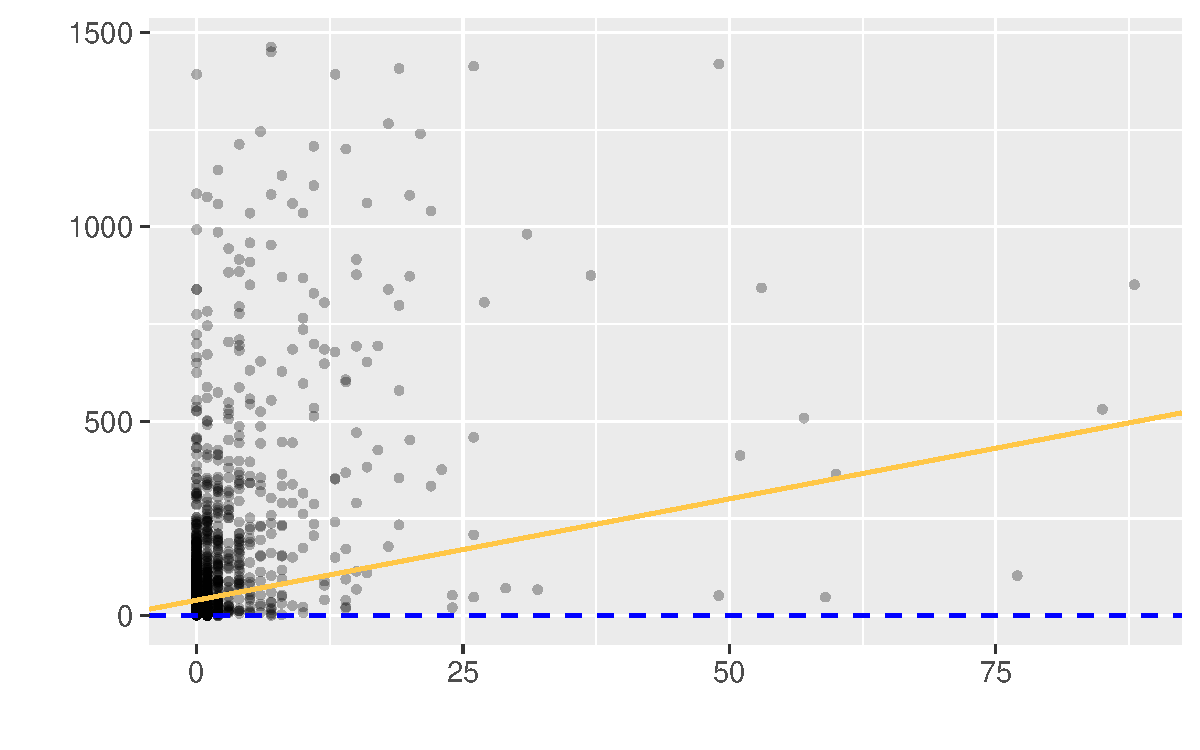
\includegraphics[page=1,scale=0.3]{../hypotheses/lm_issues_model_5_6.pdf}
  \captionof{figure}{Residual Projects \newline (Model 1.2.5 - 1.2.6)}
  \label{fig:hyp1_issue_model_5-6}
\end{minipage}
\begin{minipage}{.5\textwidth}
	\centering
	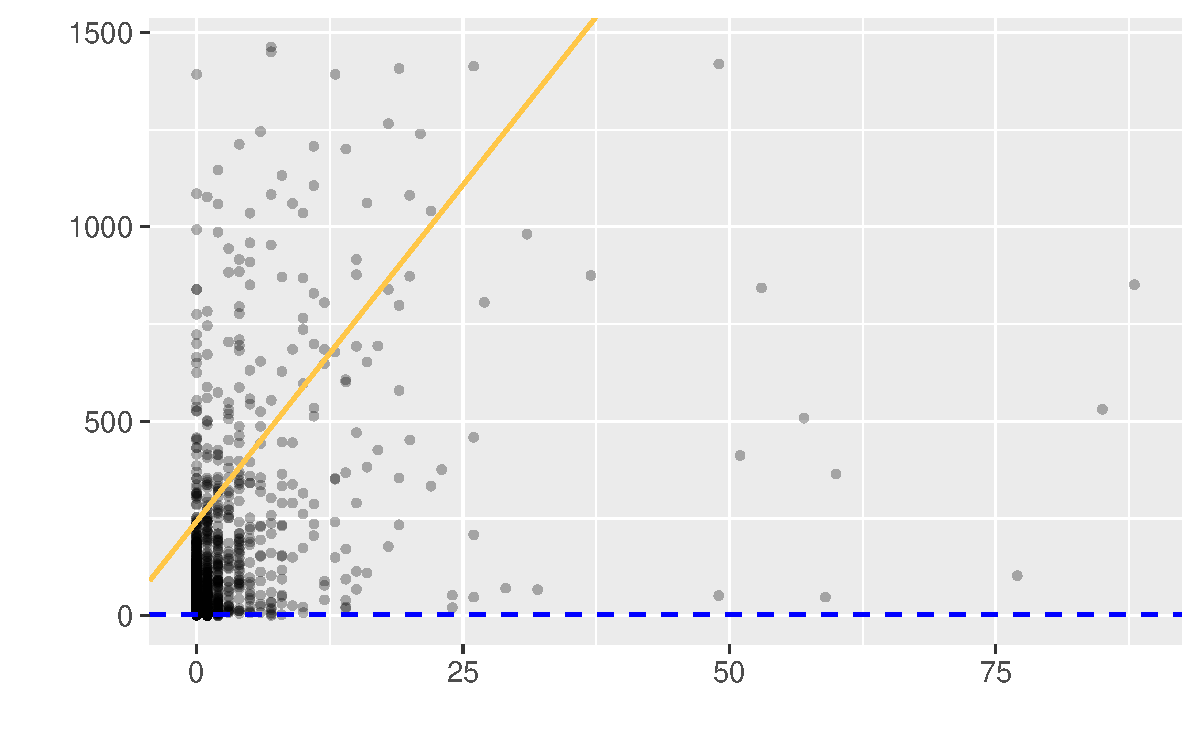
\includegraphics[page=1,scale=0.3]{../hypotheses/lm_issues_model_7_8.pdf}
  \captionof{figure}{Older Top Projects \newline (Model 1.2.7 - 1.2.8)}
  \label{fig:hyp1_issue_model_7-8}
\end{minipage}

\vspace{20 pt}

\begin{minipage}{.5\textwidth}
	\centering
	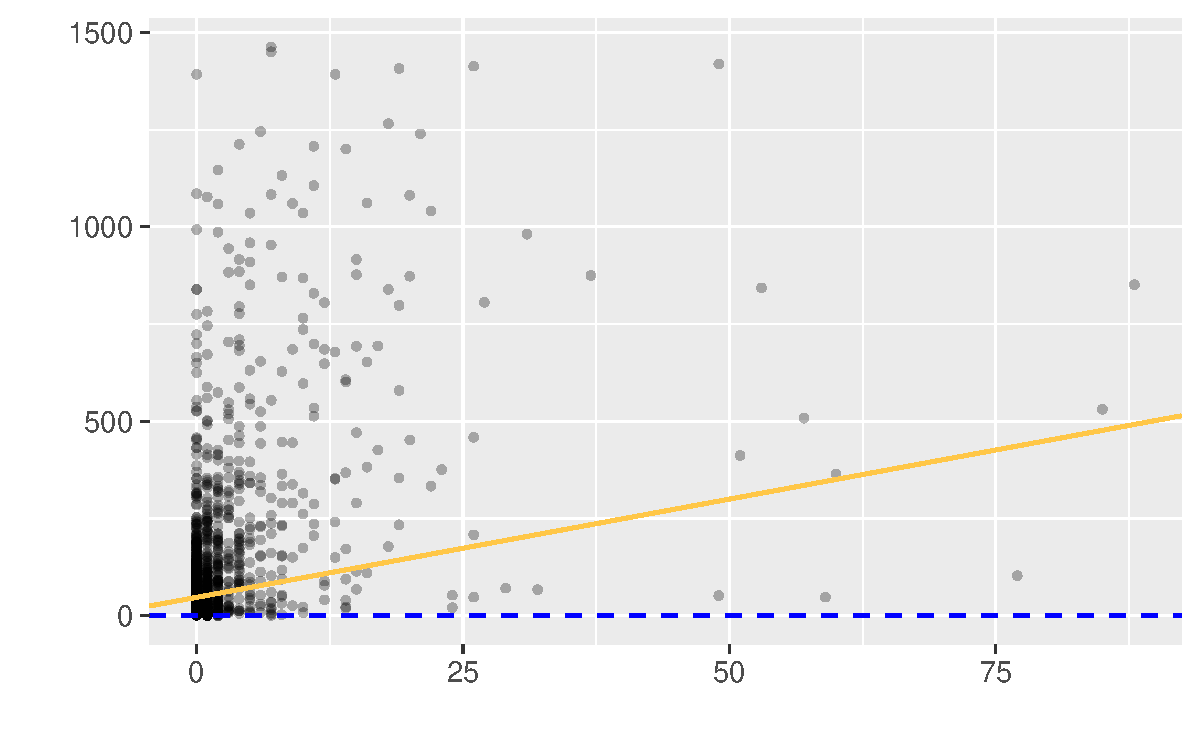
\includegraphics[page=1,scale=0.3]{../hypotheses/lm_issues_model_9_10.pdf}
  \captionof{figure}{Older Residual Projects \newline (Model 1.2.9 - 1.2.10)}
  \label{fig:hyp1_issue_model_9-10}
\end{minipage}
\begin{minipage}{.5\textwidth}
	\centering
	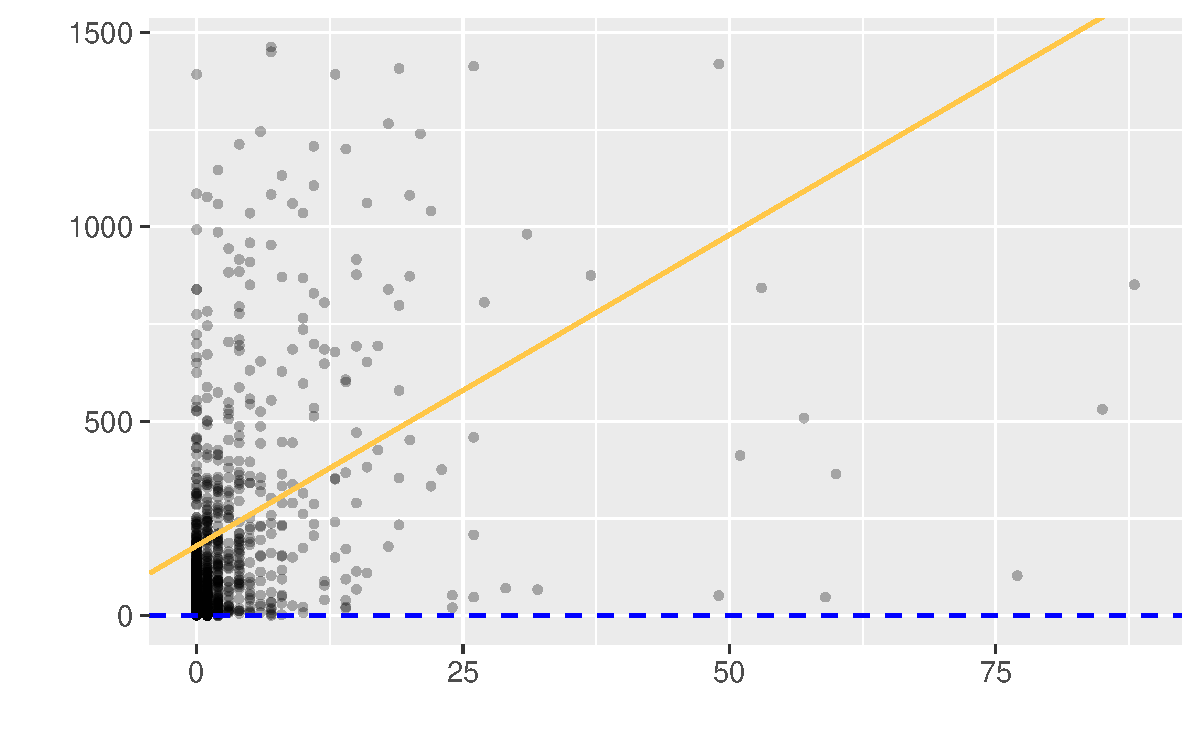
\includegraphics[page=1,scale=0.3]{../hypotheses/lm_issues_model_11_12.pdf}
  \captionof{figure}{Younger Top Projects \newline (Model 1.2.11 - 1.2.12)}
  \label{fig:hyp1_issue_model_11-12}
\end{minipage}

\vspace{20 pt}

\begin{minipage}{.5\textwidth}
	\centering
	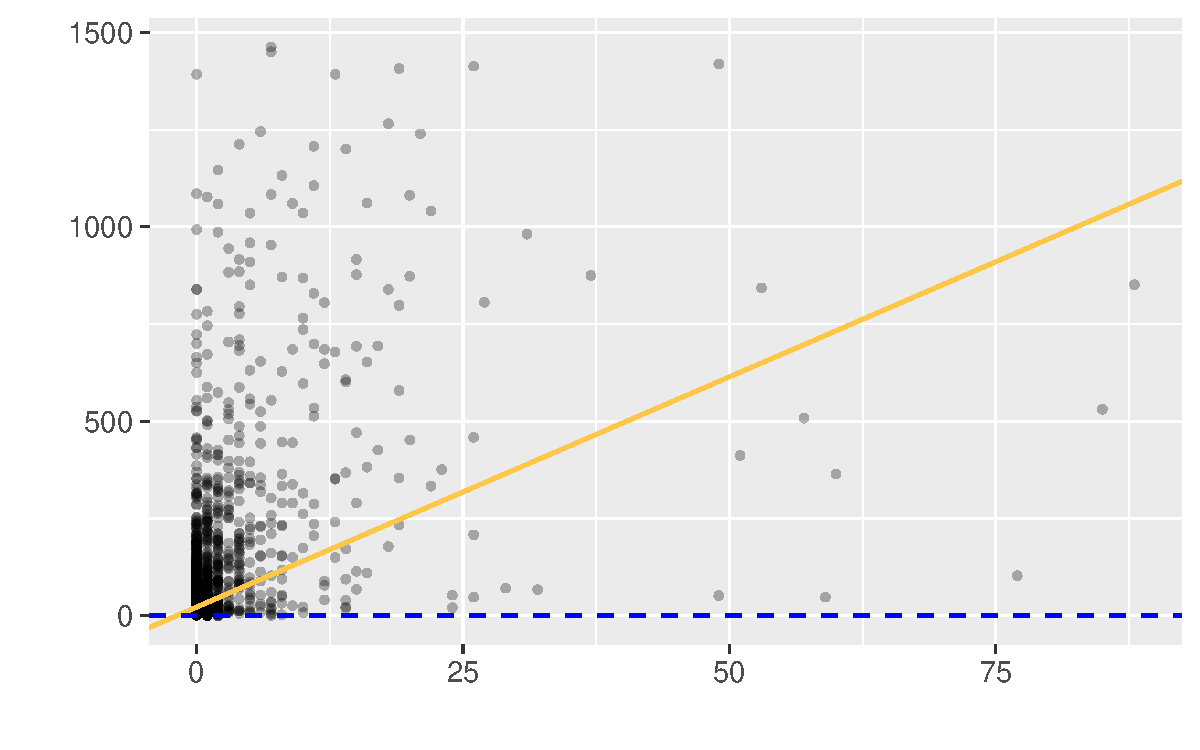
\includegraphics[page=1,scale=0.3]{../hypotheses/lm_issues_model_13_14.pdf}
  \captionof{figure}{Younger Residual Projects \newline (Model 1.2.13 - 1.2.14)}
  \label{fig:hyp1_issue_model_13-14}
\end{minipage}


\subsection{Plots for H 1.2.2}
\label{sec:h_1.2.2_plots}

See page \pageref{sec:lm_plots_description} and \pageref{sec:h1.2.2_models} for explanation of slopes and axes.
\vspace{20 pt}

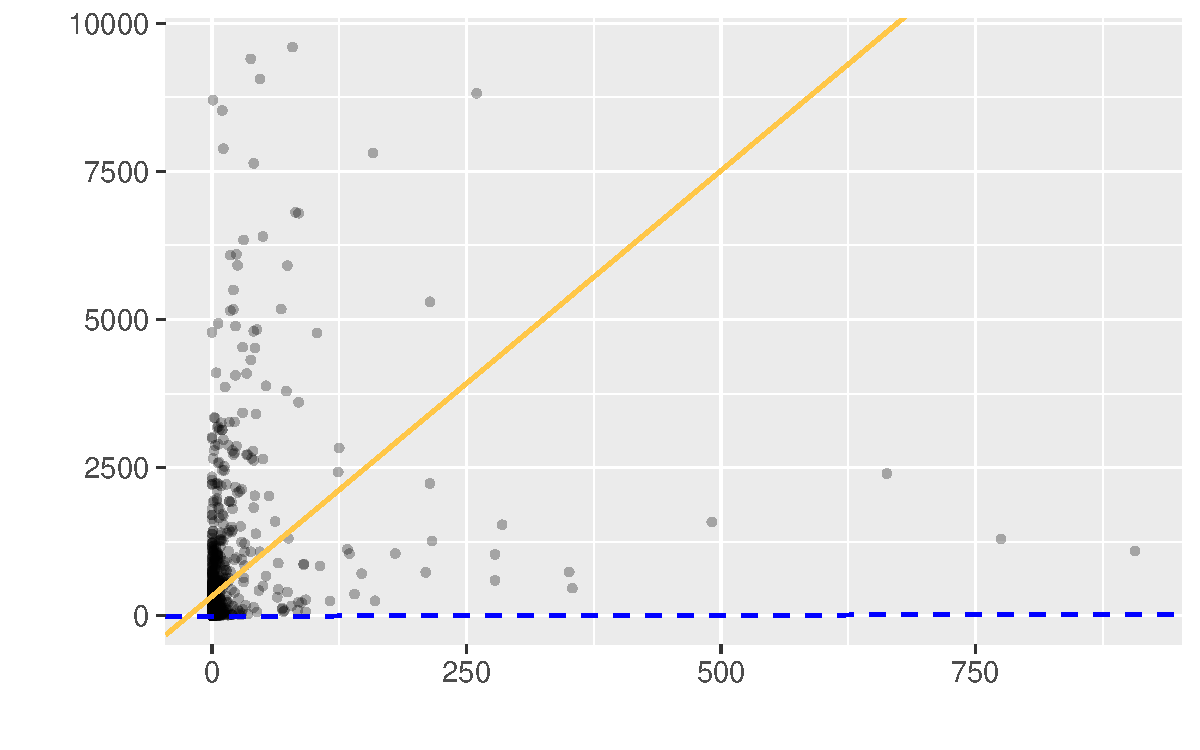
\includegraphics[page=1,scale=0.7]{../hypotheses/h1_issue_comments_all.pdf}
\captionof{figure}{Comments of Issues (Model 1.3.3- 1.3.4)}
\label{fig:hyp1_issuecomments_top_model_3}
\vspace{20 pt}
\begin{minipage}{.5\textwidth}
	\centering
	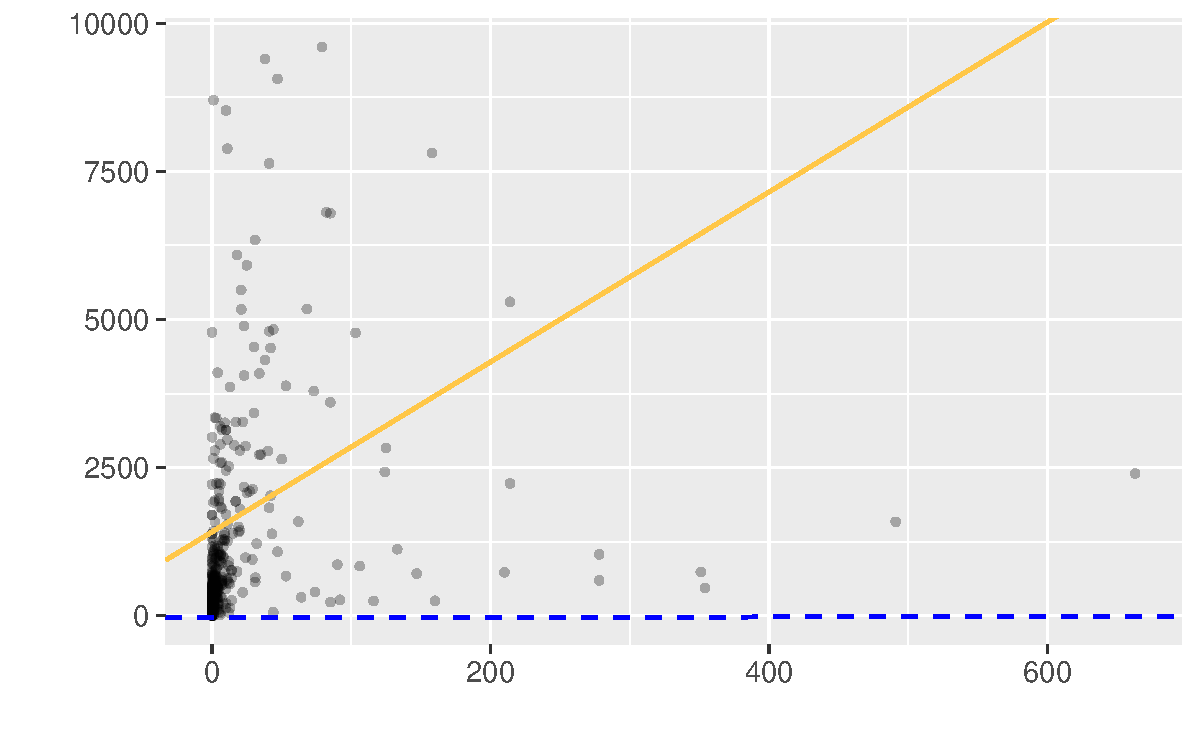
\includegraphics[page=1,scale=0.3]{../hypotheses/h1_issue_comments_top.pdf}
  \captionof{figure}{Comments of Issues \newline (Model 1.3.3- 1.3.4)}
  \label{fig:hyp1_issuecomments_residual_model_3}
\end{minipage}
\begin{minipage}{.5\textwidth}
	\centering
	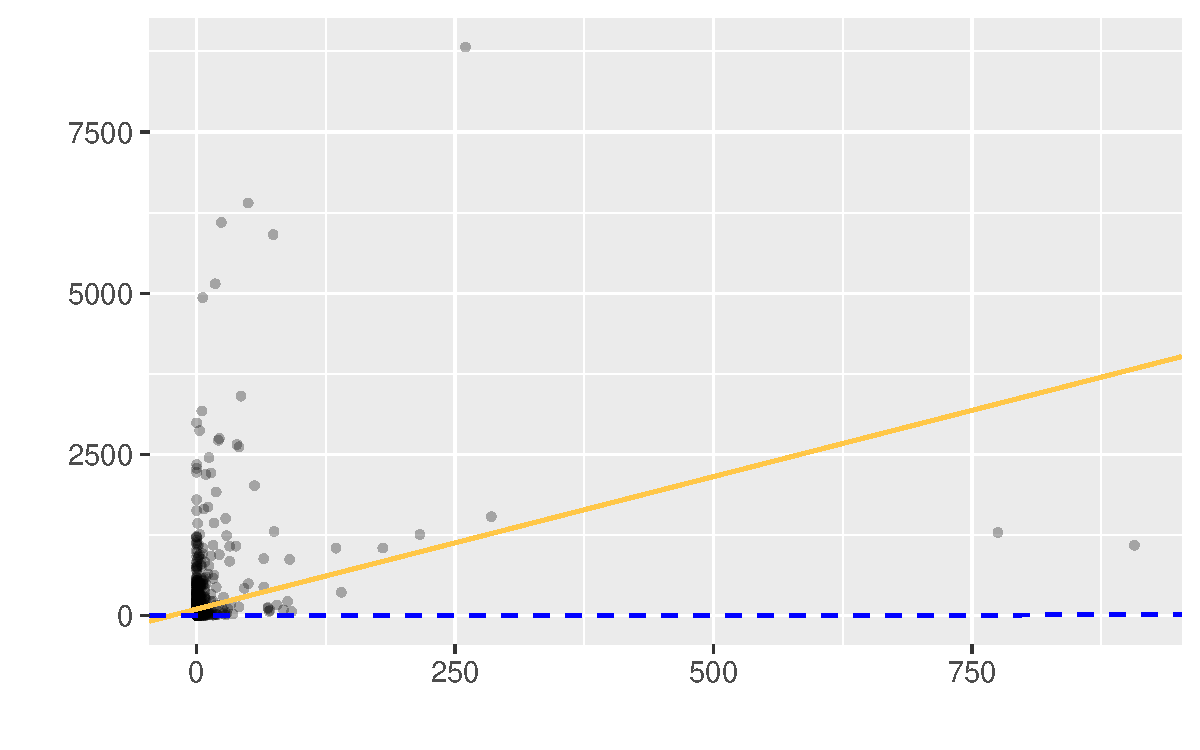
\includegraphics[page=1,scale=0.3]{../hypotheses/h1_issue_comments_residual.pdf}
  \captionof{figure}{Comments of Issues \newline (Model 1.3.5- 1.3.6)}
  \label{fig:hyp1_issuecomments_residual_model_3}
\end{minipage}
